%\documentclass[UTF8]{book} % 使用book文档类型格式排版
\usepackage{ctex}  %加载包,因为我们在用中文写文档,所以必须加载这个包,否则不支持中文

%加入了一些针对XeTeX的改进并且加入了 \XeTeX 命令来输入漂亮的XeTeX logo
\usepackage{xltxtra}
%启用一些LaTeX中的功能
\usepackage{xunicode}

\usepackage{multicol}  %加载包
\usepackage{amsmath} % 调用公式宏包
\usepackage{amssymb} % 数学符号生成命令
\usepackage{array} % 数组和表格制作
\usepackage{booktabs} % 绘制水平表格线
\usepackage{calc} %四则运算
\usepackage{caption} % 插图和表格标题格式设置
\usepackage{fancyhdr} % 页眉页脚设置
\usepackage{graphicx} % 调用插图宏包
\usepackage{multicol} % 多栏排版
\usepackage{titlesec} % 章节标题格式设置

%%%% 目录样式 %%%%
\usepackage{titletoc}
\titlecontents{chapter}[1pt]{\vspace{.5\baselineskip}\bfseries}
    {{\thecontentslabel}\quad}{}
    {\hspace{.5em}\titlerule*[10pt]{$\cdot$}\contentspage}
\titlecontents{section}[2em]{\vspace{.25\baselineskip}\bfseries}
    {\thecontentslabel\quad}{}
    {\hspace{.5em}\titlerule*[10pt]{$\cdot$}\contentspage}

\usepackage{color}
\usepackage{xcolor} % 颜色处理
%\usepackage{indentfirst} % 自动首行缩进
%\setlength{\parindent}{2.22em} % 设置首行缩进的距离
% 设置超链接颜色
\usepackage[colorlinks=true,linkcolor=black,urlcolor=black,citecolor=black]{hyperref} % 根据章节标题生成PDF书签

%%%% 版面 %%%%
\usepackage[top=0.5in,bottom=0.5in,left=1.25in,right=0.8in]{geometry}
% 设置行距
\linespread{1}
\usepackage{lscape}
\usepackage{listings} %插入代码,代码页需要加入[fragile]
\usepackage{xeCJK}

%\usepackage[slantfont,boldfont]{xeCJK} % 允许斜体和粗体

%%%% fontspec 宏包 %%%%
\usepackage{fontspec}
% 指定字体
%\setmonofont[Mapping={}]{Monaco}	%英文引号之类的正常显示,相当于设置英文字体
%\setsansfont{Monaco} %设置英文字体 Monaco, Consolas,  Fantasque Sans Mono
%\setmainfont{Monaco} %设置英文字体
% \setCJKmainfont{方正兰亭黑简体}  %中文字体设置
% \setCJKsansfont{华康少女字体} %设置中文字体
% \setCJKmonofont{华康少女字体} %设置中文字体

%%%%%%%%%% 图形支持宏包 %%%%%%%%%%
\usepackage{graphicx}                % 嵌入png图像
\usepackage{color,xcolor}            % 支持彩色文本、底色、文本框等
%\usepackage{subfigure}
%\usepackage{epsfig}                 % 支持eps图像
%\usepackage{picinpar}               % 图表和文字混排宏包
%\usepackage[verbose]{wrapfig}       % 图表和文字混排宏包
%\usepackage{eso-pic}                % 向文档的部分页加n副图形, 可实现水印效果
%\usepackage{eepic}                  % 扩展的绘图支持
%\usepackage{curves}                 % 绘制复杂曲线
%\usepackage{texdraw}                % 增强的绘图工具
%\usepackage{treedoc}                % 树形图绘制
%\usepackage{pictex}                 % 可以画任意的图形
%\usepackage{hyperref}

%\setCJKmainfont{Kai}   % 设置缺省中文字体
%\setCJKmonofont{Hei}   % 设置等宽字体
%\setmainfont{Optima}   % 英文衬线字体
%\setmonofont{Monaco}   % 英文等宽字体
%\setsansfont{Trebuchet MS} % 英文无衬线字体

\makeatletter
\providecommand*\input@path{}
\newcommand\addinputpath[1]{
\expandafter\def\expandafter\input@path
\expandafter{\input@path{#1}}}
\addinputpath{body/}
\makeatother

\definecolor{keywordcolor}{rgb}{0.8,0.1,0.5}
\lstset{language=C++, %用于设置语言为C++
    numbers=left, %设置行号位置
    numberstyle=\tiny, %设置行号大小
    keywordstyle=\color{keywordcolor} \bfseries,
    identifierstyle=,
    basicstyle=\ttfamily,
    commentstyle=\color{blue} \textit, %注释颜色
    stringstyle=\ttfamily,
    showstringspaces=false,
    frame=shadowbox, %边框
    %frame = single,
    tabsize=2, %设置tab空格数
    showspaces=false, %不显示空格
    escapeinside=``, %逃逸字符(1左面的键),用于显示中文
    %breaklines, %自动折行
    captionpos=b
}
%\begin{document}

\chapter{图论}

\section{最小生成树}

\subsection{$Kruskal\ Algorithm$}
时间复杂度:$O(m*\log m)$
\begin{lstlisting}
int Kruskal()
{ // 结构体存边
	sort(edge, edge + m);
	int res = 0;
	for (int i = 0; i < m; ++i) {
		int u = edge[i].u, v = edge[i].v, w = edge[i].w;
		int fu = find(u), fv = find(v);
		if (fu != fv) {
			fa[fu] = fv;
			res += w;
		}
	}
	return res;
}
\end{lstlisting}

\subsection{$Prim\ Algorithm$}
时间复杂度:$O(n^2)$

\begin{lstlisting}
int Prim()
{
	int res = 0;
	vis[0] = 1; // 以任意点为起点都可以
	for (int i = 0; i < n; ++i) {
		way[i] = dis[i][0]; // 二维数组存边
		fa[i] = 0; //用于标记每个点所用到的边的另一端点编号
	}
	vis[0] = 1, fa[0] = -1;
	for (int i = 1; i < n; ++i) {
		int Min = inf, id;
		for (int j = 0; j < n; ++j) {
			if (!vis[j] && way[j] < Min) { // 未连通点中找最近的点
				Min = way[j], id = j;
			}
		}
		vis[id] = 1; // 标记已连通
		res += Min;
		if (fa[id] != -1) { // 记录用到的边
			vec[id].push_back(fa[id]);
			vec[fa[id]].push_back(id);
		}
		for (int j = 0; j < n; ++j) { // 更新
			if (!vis[j] && dis[id][j] < way[j]) {
				way[j] = dis[id][j];
				fa[j] = id;
			}
		}
	}
	return res;
}
\end{lstlisting}

\clearpage
\section{拓扑排序}

拓扑排序$(Topological\  Sorting)$主要用来解决:$A\rightarrow B$表示活动$A$必须在活动$B$之前完成。请给出一个合理的活动顺序。也可以用拓扑排序来判断图中是否存在环。 \\
过程:
\begin{itemize}
\item 记录每个点的入度。
\item 将入度为0的顶点加入队列。
\item 依次对入度为0的点进行删边操作,同时将新得到的入度为零的点加入队列。
\item 重复上述操作,直至队列为空。
\end{itemize}
选择度为0的点不同,一般拓扑排序也就不同。 \\
但要注意字典序最小的拓扑排序和\underline {让编号为1的人尽量小,然后让编号为2的人尽量小,让编号为3的人尽量小……}的区别。 \\
前者是将队列中度为0的点,利用优先队列小元素先出,这样可以字典序最小。 \\
而后者等价于\\
\underline {对于编号为1:除了强制有优先关系的,在他前面不应该有其他的点} \\
\underline {对于编号为2:在满足编号1的条件下和本身存在优先关系的,在他前面不应该有其他的点}\\
\underline {.....}
举个例子:\\
$n=4,m=2$ \\
$3>1$ \\
$2>4$ \\
符合前者的编号顺序应该是:$2,3,1,4$(字典序最小) \\
符合后者的编号顺序应该是:$3,1,2,4$(编号1尽量靠前) \\
我们来考虑这个排序在多解时的最终状态的性质:\underline {编号大的靠后} \\
那么我们可以\underline {反向建图},先将编号大的排列出来,然后将可能解锁的大编号也加进优先队列【并且优先队列是大元素先出】,依次排列就好了。 \\

\begin{lstlisting}
//普通的拓扑排序模板
int degree[MAX_N], ans[MAX_N];
vector<int> vec[MAX_N];
queue<int> que;

int TopoSort(int n)
{
    while(!que.empty()) que.pop();
    for(int i = 0; i < n; ++i) { // 编号 0--n
        if(degree[i] == 0) que.push(i);
    }
    int total = 0, flag = 0;
    while(!que.empty()) {
        if(flag == 0 && que.size() > 1) flag = 1; // 有多个度为 0 的点
        int cur = que.front();
        que.pop();
        ans[total++] = cur; //记录序列
        for(int i = 0; i < vec[cur].size(); ++i) {
            int to = vec[cur][i];
            degree[to]--;
            if(degree[to] == 0) { //度为 0 的点入队列
                que.push(to);
            }
        }
    }
    if(flag == 0 && total == n) return 1; // 唯一确定
    for(int i = 0; i < n; ++i) {
        if(degree[i] > 0) return -1; //有环,冲突
    }
    return 0; //不能确定
}
\end{lstlisting}

\clearpage
\section{欧拉回路}

\subsection{判断}
欧拉回路:从图的某一个顶点出发,图中每条边走且仅走一次,最后回到出发点。\\
欧拉路径:从图的某一个顶点出发,图中每条边走且仅走一次,最后到达某一个点。 \\

以下所有判断都还有一个限制条件:图连通[并查集或者dfs或者bfs判断]。 \\
无向图欧拉回路判断:所有顶点的度数都为偶数。 \\
有向图欧拉回路判断:所有顶点的出度与入度相等。 \\
无向图欧拉路径判断:至多有两个顶点的度数为奇数,其他顶点的度数为偶数。 \\
有向图欧拉路径判断:至多有两个顶点的入度和出度绝对值差1(若有两个这样的顶点,则必须其中一个出度大于入度,另一个入度大于出度),其他顶点的入度与出度相等。 \\

\subsection{$n$个点和$m$条无向边的图,每条边仅可遍历一次,求图中欧拉路径的条数}
\underline {[HDU 3081  $n\leq 10^5,m\leq 2*10^{5}$]}

相当于每次可以从图中取走一个环或者环连环或者一个单链,求最少需要多少次能把所有边取完。考虑每个连通块(并查集实现)。因为是无向边,如果所有点的度数都是偶数,那么只需要一次就可以把这个连通块遍历完。如果连通块内有$k$个度数为奇数的点,那么需要$\frac{k+1}{2}$次才能把这个连通块遍历完。注意排除孤立点的情况。
\begin{lstlisting}
const int MAX_N = 100010;

int n, m;
int fa[MAX_N], degree[MAX_N], num[MAX_N];
set<int> s;
set<int>:: iterator it;

void init()
{
	for (int i = 0; i <= n; ++i) {
		num[i] = degree[i] = 0;
		fa[i] = i;
	}
}

int find(int x)
{
	return fa[x] == x ? x : fa[x] = find(fa[x]);
}

void wyr()
{
	s.clear();
	for (int i = 1; i <= n; ++i) {
		int fi = find(i);
		s.insert(fi);
		if (degree[i] & 1) num[fi]++;
	}
	int ans = 0;
	for (it = s.begin(); it != s.end(); ++it) {
		int x = (*it);
		if (num[x]) ans += (num[x] + 1) / 2;
		else if (degree[x]) ans++; //排除孤立点
	}
	printf("%d\n", ans);
	
}

int main()
{
	while (~scanf("%d%d", &n, &m)) {
		init();
		for (int i = 0; i < m; ++i) {
			int u, v;
			scanf("%d%d", &u, &v);
			degree[u]++, degree[v]++;
			int fu = find(u), fv = find(v);
			fa[fu] = fv;
		}
		wyr();
	}
	return 0;
}
\end{lstlisting}

\subsection{单词拼接,字典序最小}
\underline{[POJ 2337]} \\
给$n\leq 1000$个只含小写字母的单词,如果一个单词A的首字母是单词B的尾字母那么A可以拼接在B后面,问这$n$ 个单词能否拼成一个新的单词,如果可以输出字典序最小的答案。 \\

\begin{lstlisting}
const int MAX_N = 1010;

int T, n, total, m;
int in[30], out[30], fa[30], head[30], used[30];
int sta[MAX_N];

struct Dict {
	char s[25];
	bool operator < (const Dict& rhs) const {
		return strcmp(s, rhs.s) >= 0;
    // 保证链式前向星遍历边的时候先遍历“小”的单词
	}
} dict[MAX_N];

struct Edge {
	int v, next, vis;
} edge[MAX_N];

void AddEdge(int u, int v)
{
	edge[total].v = v, edge[total].vis = 0;
	edge[total].next = head[u];
	head[u] = total++;
}

int find(int x)
{
	return fa[x] == x ? x : fa[x] = find(fa[x]);
}

void BuildEdge()
{
	total = 0;
	sort(dict, dict + n);
	memset(in, 0, sizeof (in));
	memset(out, 0, sizeof (out));
	memset(used, 0, sizeof (used));
	memset(head, -1, sizeof (head));
	for (int i = 0; i < 30; ++i) { fa[i] = i; }
	for (int i = 0; i < n; ++i) {
		int len = strlen(dict[i].s);
		int u = dict[i].s[0] - 'a', v = dict[i].s[len - 1] - 'a';
		AddEdge(u, v); // 每个单词看成一个有向边
		used[u] = used[v] = 1;
		out[u]++, in[v]++;
		int fu = find(u), fv = find(v);
		if (fu != fv) {
			fa[fu] = fv;
		}
	}
}

int check()
{
	int root = -1, cnt1 = 0, cnt2 = 0, st;
	for (int i = 0; i < 26; ++i) {
		if (used[i] == 0) continue;
		if (root == -1) root = find(i); // 判断连通分量个数
		else if (root != find(i)) return -1;

		if (in[i] - out[i] == 1) cnt1++; // 入度恰比出度大1
		if (out[i] - in[i] == 1) cnt2++, st = i; // 出度恰比入度大1
		if (abs(in[i] - out[i]) >= 2) return -1;
	}
	// 有向图欧拉回路判断
	if ((cnt1 == 1 && cnt2 == 1) || (cnt1 == 0 && cnt2 == 0)) {
		if (cnt1 == 1) return st;
		for (int i = 0; i < 26; ++i) {
			if (out[i] > 0) return i; // 找到字典序最小的起点
		}
	} else return -1;
}

void Euler(int u, int id)
{	
	for (int i = head[u]; i != -1; i = edge[i].next) {
		if (edge[i].vis) continue;
		edge[i].vis = 1;
		Euler(edge[i].v, i);
	}
	if (id != -1) sta[m++] = id;
}

void wyr()
{	
	BuildEdge();
	int st = check();
	if (st == -1) {
		printf("***\n");
		return;
	}
	m = 0;
	Euler(st, -1);
	for (int i = n - 1; i >= 0; --i) { // 逆序输出
		printf("%s", dict[sta[i]].s);
		if (i) printf("."); // 每个单词用.间隔
		else printf("\n");
	}
}

int main()
{
	int T;
	scanf("%d", &T);
	while (T--) {
		scanf("%d", &n);
		for (int i = 0; i < n; ++i) {
			scanf("%s", dict[i].s);
		}
		wyr();
	}
	return 0;	
}
\end{lstlisting}

\subsection{正向反向两次遍历所有边,路径输出}
\underline {[POJ 2230]} \\
$n\leq 10000$个点和$m\leq 50000$条无向边的图,要求正向和方向两次遍历所有的边,输出$2*m+1$个顶点编号表示遍历顺序,保证有解。\\

直接从任意起点遍历所有的边。必须先逆序保存遍历的顶点编号,也就是必须先dfs再保存顶点编号。\\
参考样例:
\begin{center}
$n = 3, m = 2: (2, 3),(1, 2)$
\end{center}
如果先保存顶点编号再dfs的话结果是:
\begin{center}
1 2 1 3 2 (实际上应是:1 2 3 2 1)
\end{center}
这和链式前向星的建边顺序有关。

\begin{lstlisting}
const int MAX_N = 10010;
const int MAX_M = 50010;

int n, m, total, cnt;
int head[MAX_N], res[MAX_M * 2];

struct Edge {
	int v, next, vis;
} edge[MAX_M * 2];

inline void AddEdge(int u, int v)
{
	edge[total].v = v;
	edge[total].next = head[u];
	edge[total].vis = 0;
	head[u] = total++;
}

void dfs(int u)
{
	for (int i = head[u]; i != -1; i = edge[i].next) {
		if (edge[i].vis == 0) {
			edge[i].vis = 1;
			dfs(edge[i].v);
			res[cnt++] = edge[i].v;
            // 必须先逆序保存结果
		}
	}
}

int main()
{
	while (~scanf("%d%d", &n, &m)) {
		memset(head, -1, sizeof (head));
		total = cnt = 0;
		for (int i = 0; i < m; ++i) {
			int u, v;
			scanf("%d%d", &u, &v);
			AddEdge(u, v);
			AddEdge(v, u);
		}
		dfs(1); // 选取任意起点
		res[cnt++] = 1; // 起点
		for (int i = cnt - 1; i >= 0; --i) { // 逆序输出
			printf("%d\n", res[i]);
		}
	}
	return 0;
}
\end{lstlisting}

\clearpage
\section{dfs序}
\subsection{CF 396 C}
给一个$n\leq 3*10^5$个结点,根为1的树。初始时每个节点的值均为0,有$Q\leq 3*10^5$种操作:
\begin{itemize}
\item $1\ v\ x\ k:$对于以$v$为根的子树,如果结点$i$到$v$的距离为$dis$,那么$i$的权值将增加$x-dis*k$,距离就是路径上边的数量,$v$结点的权值将增加$x$。
\item $2\ v:$查询$v$结点的权值
\end{itemize}
对于每次查询输出答案,结果模$1e9+7$。 \\

把以$v$为根的子树结点转化成$dfs$序,并且得到每个结点的深度$depth[v]$。然后对于每次第1种操作,以$v$为根的子树上结点$i$相当于权值增加了
$$
x-(depth[i]-depth[v])*k=x+depth[v]*k-depth[i]*k
$$
也就是对于$dfs$序上的区间$[left[v],right[v]]$上的每一个结点$i$都需要增加$x+depth[v]*k$,然后减掉$depth[i]*k$,把加减的权值看成两颗树状数组,相当于区间更新,单点查询,维护一下即可。 \\
时间复杂度:$O(Q*\log n)$
\begin{lstlisting}
const int MAX_N = 300010;
const ll mod = (ll)(1e9) + 7;

int n, d = 0, Q;
int depth[MAX_N], left[MAX_N], right[MAX_N];
ll add[MAX_N], sub[MAX_N];
vector<int> son[MAX_N];

void dfs(int u, int k) {
	left[u] = ++d;
	depth[u] = k;
	int size = son[u].size();
	for (int i = 0; i < size; ++i) {
		dfs(son[u][i], k + 1);
	}
	right[u] = d;
}

inline int lowbit(int x) { return x & -x; }

void update(ll *bit, int x, ll value) {
	value %= mod;
	if (value < 0) value += mod;
	for (int i = x; i <= n; i += lowbit(i)) {
		bit[i] += value;
		if (bit[i] >= mod) bit[i] -= mod;
	}
}

ll query(ll *bit, int x) {
	ll ret = 0;
	for (int i = x; i > 0; i -= lowbit(i)) {
		ret += bit[i];
		if (ret >= mod) ret -= mod;
	}
	return ret;
}

int main() {
	scanf("%d", &n);
	for (int i = 2; i <= n; ++i) {
		int t;
		scanf("%d", &t);
		son[t].push_back(i);
	}
	dfs(1, 1);
	scanf("%d", &Q);
	while (Q--) {
		int type, id, x, k;
		scanf("%d", &type);
		if (type == 1) {
			scanf("%d%d%d", &id, &x, &k);
			ll value = 1ll * depth[id] * k % mod + x;
			update(add, left[id], value);
			update(add, right[id] + 1, -value);
			update(sub, left[id], k);
			update(sub, right[id] + 1, -k);
		} else {
			scanf("%d", &id);
			ll ans = (query(add, left[id]) - query(sub, left[id]) * depth[id] % mod) % mod;
			if (ans < 0) ans += mod;
			printf("%lld\n", ans);
		}
	}
	return 0;
}
\end{lstlisting}

\clearpage
\section{LCA}

\subsection{暴力求解}
记节点$v$到根的深度为$depth[v]$。那么如果节点$w$是$u$和$v$的公共祖先的话,让$u$向上走$depth[u]-depth[w]$步,让$v$向上走$depth[v]-depth[w]$ 步,都将走到$w$。因此,首先让$u$和$v$中较深的一个向上走$|depth[u]-depth[v]|$步,再一起一步步向上走,直到走到同一个节点即是$LCA$。 \\
时间复杂度:$dfs$:$O(n)$,单次查询:$O(n)$
\begin{lstlisting}
// 链式前向星建边,单向边
void dfs(int u, int p, int cur)
{
	fa[u] = p, depth[u] = cur;
	for (int i = head[u]; i != -1; i = edge[i].next) {
		dfs (edge[i].v, u, cur + 1);
	}
}

int LCA(int u, int v)
{
	while (depth[u] > depth[v]) u = fa[u];
	while (depth[v] > depth[u]) v = fa[v];
	while (u != v) {
		u = fa[u];
		v = fa[v];
	}
	return u;
}
主函数中:
for (int i = 1; i <= n; ++i) {
	if (in[i] == 0) {
		root = i; // 找到入度为 0 的根节点
		break;
	}
}
dfs (root, -1, 0);
调用:LCA(U, V);
\end{lstlisting}

\subsection{二分搜索}
首先对于任意节点$v$,利用其父节点$parent[v][1]$信息,可以通过$parent[v][2]=parent[parent[v][1]][1]$得到其向上走两步所到的节点,再利用这一信息,又可以通过$parent[v][4]=parent[parent[v][2]][2]$得到其向上走四步所到的节点。依此类推,就能够得到其向上走$2^k$步所到的节点$parent[v][k]$。有了$k=floor(log_{2}(n))$以内的所有信息后,就可以二分搜索了。 \\
预处理$parent[v][k]$:$O(n\log n)$,单次查询:$O(\log n)$
\begin{lstlisting}
// 链式前向星建边,单向边
void dfs(int u, int p, int d)
{ // 获取每个节点的深度和直接父亲
	depth[u] = d, fa[u][0] = p;
	for (int i = head[u]; i != -1; i = edge[i].next) {
		dfs(edge[i].v, u, d + 1);
	}
}

void RMQ() // 时间复杂度: O(nlog(n))
{ // 倍增处理每个节点的祖先
	for (int k = 0; k + 1 < MAX_LOG_N; ++k) {
		for (int i = 1; i <= n; ++i) {
			if (fa[i][k] == -1) fa[i][k + 1] = -1;
			else fa[i][k + 1] = fa[fa[i][k]][k];
		}
	}	
}

int LCA(int u, int v) // 时间复杂度:O(log(n))
{
	// 先把两个节点提到同一深度
	if (depth[u] > depth[v]) swap(u, v);
	for (int k = 0; k < MAX_LOG_N; ++k) {
		if (((depth[v] - depth[u]) >> k) & 1) {
			v = fa[v][k];
		}
	}
	if (u == v) return v;
	// 二分搜索计算LCA
	for (int k = MAX_LOG_N - 1; k >= 0; --k) {
		if (fa[u][k] != fa[v][k]) {
			u = fa[u][k];
			v = fa[v][k];
		}
	}
	return fa[u][0];
}
// 主函数中需要: memset(fa, -1, sizeof(fa)); fa[MAX_N][MAX_LOG_N]
for (int i = 1; i <= n; ++i) {
	if (in[i] == 0) {
		root = i;
		break;
	}
}
dfs(root, -1, 0);
RMQ();
printf("%d\n", LCA(u, v));
\end{lstlisting}

\subsection{基于RMQ的算法}
将树转为从根$DFS$标号后得到的序列处理。 \\
首先按从根$DFS$访问的顺序得到顶点序列$vis[i]$和对应的深度$depth[i]$。对于每个顶点$v$,记其在$vis[]$中首次出现的下标为$id[v]$。而$LCA(u,v)$ 就是访问$u$之后到访问$v$之前所经过的节点中离根最近的那个,假设$id[u]\leq id[v]$,那么有:
\begin{center}
$LCA(u,v)=vis[k]$,其中$k$是所有$id[u]\leq i \leq id[v]$中$depth[i]$最小的$i$
\end{center}
预处理:$O(n\log n)$,单次查询:$O(1)$
\begin{lstlisting}
int vis[MAX_N * 2], depth[MAX_N * 2], dp[MAX_N * 2][20];
// 需要开两倍空间
int head[MAX_N], in[MAX_N], id[MAX_N];
// 链式前向星建边,单向边
void dfs(int u, int p, int d, int& k)
{
	vis[k] = u; // dfs 访问顺序
   	id[u] = k; // 节点在 vis 中首次出现的下标
	depth[k++] = d; // 节点对应的深度
	for (int i = head[u]; i != -1; i = edge[i].next) {
		int v = edge[i].v;
		if (v == p) continue;
		dfs(v, u, d + 1, k); // 递归访问子节点
		vis[k] = u; // 再次访问
		depth[k++] = d; // 标记 vis 的深度
	}
}

void RMQ(int root) // 处理区间深度最小值,保存最小值的下标
{ // 就是区间左右端点最近公共祖先的下标,即: vs[Min] = LCA
	int k = 0;
	dfs(root, -1, 0, k);
	int m = k; // m = 2 * n - 1
	int e = (int)(log2(m + 1.0)); // 区间长度 m + 1
	for (int i = 0; i < m; ++i) dp[i][0] = i;
	for (int j = 1; j <= e; ++j) {
		for (int i = 0; i + (1 << j) - 1 < m; ++i) {
			int nxt = i + (1 << (j - 1));
			if (depth[dp[i][j - 1]] < depth[dp[nxt][j - 1]]) {
				dp[i][j] = dp[i][j - 1];
			} else {
				dp[i][j] = dp[nxt][j - 1];
			}
		}
	}
}

int LCA(int u, int v)
{
	int left = min(id[u], id[v]), right = max(id[u], id[v]);
	int k = (int)(log2(right - left + 1.0)); // 区间长度,注意用log2!
	int pos, nxt = right - (1 << k) + 1; // nxt 分界点
	if (depth[dp[left][k]] < depth[dp[nxt][k]]) {
		pos = dp[left][k];
	} else {
		pos = dp[nxt][k];
	}
	return vis[pos];
}
// 主函数中:
RMQ(root);
printf("%d\n", LCA(u, v));
\end{lstlisting}

\subsection{Tarjan算法}
算法从根节点$root$开始搜索,每次递归搜索所有的子树,然后处理跟当前根节点相关的所有查询。 \\
用集合表示一类节点,这些节点跟集合外的点的$LCA$都一样,并把这个$LCA$设为这个集合的祖先。当搜索到节点$x$时,创建一个由$x$本身组成的集合,这个集合的祖先为$x$自己。然后递归搜索$x$的所有儿子节点。当一个子节点搜索完毕时,把子节点的集合与$x$节点的集合合并,并把合并后的集合的祖先设为$x$。因为这棵子树内的查询已经处理完,$x$的其他子树节点跟这棵子树节点的$LCA$都是一样的,都为当前根节点$x$。
所有子树处理完毕之后,处理当前根节点$x$相关的查询。遍历$x$的所有查询,如果查询的另一个节点$v$已经访问过了,那么$x$和$v$的LCA即为$v$ 所在集合的祖先。 \\
其中关于集合的操作都是使用并查集高效完成。 \\
算法的复杂度为,$O(n)$搜索所有节点,搜索每个节点时会遍历这个节点相关的所有查询。如果总的查询个数为$Q$,则总的复杂度为$O(n+Q)$。
\begin{lstlisting}
int in[MAX_N], fa[MAX_N], cnt[MAX_N], vis[MAX_N], ancestor[MAX_N];
// fa[]: 并查集操作, cnt[i]:i 作为 LCA 的次数
// vis[]: 标记是否访问, ancestor[]: 存集合的LCA
vector<int> vec[MAX_N], query[MAX_N];
// vec[i]: 存 i 指向节点(儿子)信息, query[i]: 存需要查 i 和谁的 LCA

//采用邻接表建边,双向边
int find(int x)
{
	return fa[x] == x ? x : fa[x] = find(fa[x]);
}

void Union(int x, int y)
{
	int fx = find(x), fy = find(y);
	if (fx != fy) {
		fa[fy] = fx;
	}
}

void Tarjan(int x)
{
	for (int i = 0; i < vec[x].size(); ++i) {
		Tarjan(vec[x][i]);
		Union(x, vec[x][i]); // 注意传参和并查集合并顺序
	}
	vis[x] = 1; // 标记已经被访问
	for (int i = 0; i < query[x].size(); ++i) {
		if (vis[query[x][i]]) {
    // x 和 query[x][i] 的 LCA 是 find(query[x][i])
			cnt[find(query[x][i])]++;
		}
	}
}

void init()
{
	for (int i = 0; i <= n; ++i) {
		fa[i] = ancetor[i] = i;
		vec[i].clear();
		query[i].clear();
	}
	memset(vis, 0, sizeof(vis));
	memset(in, 0, sizeof(in));
	memset(cnt, 0, sizeof(cnt));
}
// 主函数中:
// 找到根节点
int root;
for (int i = 1; i <= n; ++i) {
	if (in[i] == 0) {
		root = i;
		break;
	}
}
Tarjan(root);
for (int i = 1; i <= n; ++i) {
	if (cnt[i]) printf("%d:%d\n", i, cnt[i]);
    // 输出每个节点作为查询的 LCA 的次数
}
\end{lstlisting}

\subsection{利用LCA获得树上任意两点距离}
先用基于RMQ算法的求LCA的方法求出LCA。记$dis[i]$为根节点到$i$节点的距离,那么$u$和$v$之间的距离就是:
 $$Ans=dis[u]+dis[v] - 2 * dis[LCA(u,v)]$$
时间复杂度:预处理:$O(n\log n)$,查询:$O(1)$
\begin{lstlisting}
int n, m, total;
int head[MAX_N], in[MAX_N], id[MAX_N], dis[MAX_N];
int vis[MAX_N * 2], depth[MAX_N * 2], dp[MAX_N * 2][20];

// 链式前向星建边
void dfs(int u, int p, int d, int& k)
{
	vis[k] = u, id[u] = k;
	depth[k++] = d;
	for (int i = head[u]; i != -1; i = edge[i].next) {
		int v = edge[i].v, w = edge[i].w;
		if (v == p) continue;
		dis[v] = dis[u] + w;
		dfs(v, u, d + 1, k);
		vis[k] = u;
		depth[k++] = d;
	}
}

void RMQ(int root)
{
	int k = 0;
	dfs(root, -1, 0, k);
	int mm = k;
	int e = (int)log2(mm + 1.0);
	for (int i = 0; i < mm; ++i) dp[i][0] = i;
	for (int j = 1; j <= e; ++j) {
		for (int i = 0; i + (1 << j) - 1 < mm; ++i) {
			int nxt = i + (1 << (j - 1));
			if (depth[dp[i][j - 1]] < depth[dp[nxt][j - 1]]) {
				dp[i][j] = dp[i][j - 1];
			} else {
				dp[i][j] = dp[nxt][j - 1];
			}
		}
	}
}

int LCA(int u, int v)
{
	int left = min(id[u], id[v]), right = max(id[u], id[v]);
	int k = (int)log2(right - left + 1.0);
	int pos, nxt = right - (1 << k) + 1;
	if (depth[dp[left][k]] < depth[dp[nxt][k]]) {
		pos = dp[left][k];
	} else {
		pos = dp[nxt][k];
	}
	return dis[u] + dis[v] - 2 * dis[vis[pos]];
}

void init()
{
	total = 0;
	memset(head, -1, sizeof(head));
	memset(vis, 0, sizeof(head));
	memset(in, 0, sizeof(in));
	memset(dis, 0, sizeof(dis));
	for (int i = 0; i <= n; ++i) { fa[i] = i; }
}

int main()
{
	while (~scanf("%d%d", &n, &m)) {
		init();
		for (int i = 0; i < m; ++i) {
			int u, v, w;
			char s[10];
			scanf("%d%d%d%s", &u, &v, &w, s);
			AddEdge(u, v, w); // 理论上单向边也可以
			// AddEdge(v, u, w);
			in[v]++;
		}
		int root;
		for (int i = 1; i <= n; ++i) {
			if (in[i] == 0) {
				root = i;
				break;
			}
		}
		RMQ(root);
		scanf("%d", &m);
		while (m--) {
			int u, v;
			scanf("%d%d", &u, &v);
			printf("%d\n", LCA(u, v));
		}
	}
	return 0;
}
\end{lstlisting}

\clearpage
\section{最小树形图}
有向图的最小生成树。

\subsection{朱刘算法}
朱-刘Edmonds算法步骤:
\begin{enumerate}
\item 找到除了$root$以为其他点的权值最小的入边。用$In[i]$记录
\item 如果出现除了$root$以为存在其他孤立的点,则不存在最小树形图
\item 找到图中所有的环,并对环进行缩点,重新编号
\item 更新其他点到环上的点的距离,如:环中的点有$(Vk1,Vk2,… ,Vki)$总共$i$个,用缩成的点叫$Vk$替代,则在压缩后的图中,其他所有不在环中点$v$到$Vk$的距离定义如下:\\
$$gh[v][Vk]=min { gh[v][Vkj]-mincost[Vkj] } (1\leq j\leq i)$$
即所有到环上点的权减去环上点的最小入边权。\\
而Vk到v的距离为\\
$$gh[Vk][v]=min { gh[Vkj][v] }  (1\leq j\leq i)$$
从环上点出发的边的边权为环上所有点到终点的边权的最小值
\item 重复3,4直到没有环为止。
\end{enumerate}

时间复杂度:$O(nm)$

\subsection{有固定根}
\underline {POJ 3164 Command Network} \\

给出$n$个点(下标从$1\sim n$)的坐标和$m$条单向边$[i,j]$表示可以从$i$点建一条边到$j$,权值是两点距离,求将这$n$个点连通的最小边权和。如果无法连通输出$"poor\ snoopy"$,否则输出最小边权和。
\begin{lstlisting}
const int MAX_N = 110;
const int MAX_M = 10010;
const double INF = 1e20;
const double eps = 1e-8;

int n, m;
int NV, NE;
// NV 和 NE 分别是结点和边个数(结点下标从 0--NV - 1, 边下标从 0-- NE - 1)
int ID[MAX_N], vis[MAX_N], pre[MAX_N];
//结点重新编号后的编号、寻找环时是否访问、结点的前驱结点
double  In[MAX_N]; //结点入度最小值

struct Point{
    double x, y;

    Point() {}
    Point(double _x, double _y) : x(_x),y(_y) {}

    double dis(const Point& rhs) const {
        return hypot(x - rhs.x, y - rhs.y);
    }
}point[MAX_N];

struct Edge{
    int u, v;
    double w;

    Edge() {}
    Edge(int _u, int _v, double _w) :u(_u), v(_v), w(_w) {}
}edge[MAX_M];

//ZLEdmonds Algorithm
double Directed_MST(int root)
{
    double res = 0, w;
    int u, v;
    while(1){
        // 1. 找最小入边
        for(int i = 0; i < NV; i++) In[i] = INF;
        //将所有结点的入度设为-1
        for(int i = 0; i < NE; i++){
            u = edge[i].u;
            v = edge[i].v;
            w = edge[i].w;
            if(u != v && w < In[v]){ //消除自环影响
                In[v] = w;
                pre[v] = u;
            }
        }
        for(int i = 0; i < NV; i++){
        //检查是否存在除 root 孤立点,若存在则不存在最小树形图
            if(i == root) continue;
            if(In[i] == INF) return -1; // i 是孤立点
        }
        // 2. 找环
        int cnt = 0; //记录所有结点重新标号后新结点数量
        memset(vis, -1, sizeof(vis));
        memset(ID, -1, sizeof(ID));
        In[root] = 0; // 将根节点入度重设为0
        for(int i = 0; i < NV; i++){ // 遍历所有结点找环
            res += In[i]; // 结果加上当前结点的最少入度
            v = i;
            while(vis[v] != i && ID[v] == -1 && v != root){
            //将 v 所在有向环(或有向单链)上的所有结点收缩为 i 结点
                vis[v] = i;
                v = pre[v];
            }
            if(v != root && ID[v] == -1){ //只有有向环时重新标号
                for(int u = pre[v]; u != v; u = pre[u]){
                //将 i 所在有向环上所有结点收缩为结点 cnt
                    ID[u] = cnt;
                }
                ID[v] = cnt++;
            }
        }
        if(cnt == 0) break;
        //只剩下了 root 所在的有向环
        for(int i = 0; i < NV; ++i){
            if(ID[i] == -1) ID[i] = cnt++;
            // root 所在有向环上结点或者其他有向环外接单链上点重新标号
        }
        // 3. 建新图
        for(int i = 0; i < NE; i++){ // 更新其他点到环上的距离
            u = edge[i].u;
            v = edge[i].v;
            edge[i].u = ID[u];
            edge[i].v = ID[v];
            if(edge[i].u != edge[i].v){ // 收缩点后不是同一结点
                edge[i].w -= In[v];
            }
        }
        NV = cnt; // 更新新图的结点数量和根节点编号
        root = ID[root];
    }
    return res;
}

int main()
{
    while(~scanf("%d%d", &n ,&m)){
        NV = n, NE = m;
        for(int i = 1; i <= n; ++i){
            scanf("%lf%lf", &point[i].x, &point[i].y);
        }
        for(int i = 0; i < m; ++i){
            int u, v;
            scanf("%d%d", &u, &v);
            if( u != v) edge[i].w = point[u].dis(point[v]);
            else edge[i].w = INF; // 消除自环影响
            edge[i].u = u - 1, edge[i].v = v - 1; // 保证结点下标从 0--NV-1
        }
        double ans = Directed_MST(0);
        if(fabs(ans + 1) <= eps) printf("poor snoopy\n");
        else printf("%.2f\n", ans);
    }
    return 0;
}
\end{lstlisting}

\subsection{无固定根}
\underline {HDU 2121 Ice\_cream’s world II}\\

有$n$个城市(编号$0--n-1)$和$m$条边需要在$n$个城市中选择一个城市作为首都,使得从首都到其他城市的都能连通 而且路径权值和要最小。如果不能找到这样的首都输出-1,否则输出最小的路径权值和和相应的首都,如果在同一最小路径权值下有多个首都选择,输出最小编号的那个。 \\

如果原图是可以生成最小树形图,因为只添加了一个新的结点$n$,且该结点n到$0\sim n-1$的边权为$(sum + 1)$($sum$原图边权和),设新图求出的最小树形图的权值和为$ans$,新图的最小树形图的权值只比原图多了连通$n$结点的边权即$sum$,那么$ans - sum$后即应为原图的最小树形图的权值和,如果大于$sum$,说明$n$结点不止和原图中的一个结点相连,所以原图不存在最小树形图。当然如果新图不存在最小树形图,原图更不可能生成最小树形图。 \\
寻找原图的最小树形图的根,如果有多解,输出最小编号根。\\
原图的最小树形图的根节点即是和$n$结点相连的那个节点所在边的编号设为$real_root$,新图的$root = n$,在寻找结点最小入弧时如果弧的起点是$root$,那么$real_root = $这条入弧的终点,这只是必要条件。考虑充分条件:如果原图的最小树形图的根只有一个解,那么这样找肯定成立。如果有多个根,那么这些根必然存在一个环上,而且环上的每个点都可以作为原图的根节点,又因为将环缩点时是将环上的所有点缩成环上最小编号点,所以找到的必然是最小编号点。还需要注意因为$real_root$是边的编号而且边的顶点信息在$ZLEdmonds$算法中是会发生变化的,所以真正的根节点是$real_root - m$.$m$是给出的边数,因为初始建边时当$i \geq m$时,$edge[i].m = i - m$,而且求出的$real_root$一定是$\geq m$)
\begin{lstlisting}
typedef long long ll;
const int MAX_N = 1010;
const int MAX_M = 11000;
const ll INF = LONG_LONG_MAX;

int n, m, NV, NE, root, real_root;
int vis[MAX_N], pre[MAX_N], ID[MAX_N];
ll In[MAX_N];

struct Edge{
    int u, v;
    ll w;

    Edge() {}
    Edge(int _u, int _v, ll _w) : u(_u), v(_v), w(_w) {}
}edge[MAX_M];

ll ZLEdmonds(int root, int NV, int NE)
{
    ll res = 0, w;
    int u, v;
    while(1){
        for(int i = 0; i < NV; i++) {
            In[i] = INF;
        }
        for(int i = 0; i < NE; i++){
            u = edge[i].u, v = edge[i].v, w = edge[i].w;
            if(u != v && w < In[v]){
                In[v] = w;
                pre[v] = u;
                if(u == root) {
                    real_root = i;
                }
            }
        }
        for(int i = 0; i < NV; i++){
            if(i != root && In[i] == INF) return -1;
        }
        int cnt = 0;
        memset(vis, -1, sizeof(vis));
        memset(ID, -1, sizeof(ID));
        In[root] = 0;
        for(int i = 0; i < NV; i++){
            res += In[i];
            v = i;
            while(v != root && vis[v] != i && ID[v] == -1){
                vis[v] = i;
                v = pre[v];
            }
            if(v != root && ID[v] == -1){
                for(u = pre[v]; u != v; u = pre[u]){
                    ID[u] = cnt;
                }
                ID[v] = cnt++;
            }
        }
        if(cnt == 0) break;
        for(int i = 0; i < NV; i++){
            if(ID[i] == -1) ID[i] = cnt++;
        }
        for(int i = 0; i < NE; i++){
            u = edge[i].u, v = edge[i].v;
            edge[i].u = ID[u], edge[i].v = ID[v];
            if(edge[i].u != edge[i].v){
                edge[i].w -= In[v];
            }
        }
        NV = cnt;
        root = ID[root];
    }
    return res;
}

int main()
{
    while(~scanf("%d%d", &n, &m)){
        NE = 0;
        ll sum = 0;
        for(int i = 0; i < m; i++){
            int u, v;
            ll w;
            scanf("%d%d%lld", &u, &v, &w);
            edge[NE++] = Edge(u, v, w);
            sum  += w;
        }
        sum++;
        for(int i = 0; i < n; i++){
            edge[NE++] = Edge(n, i, sum);
        }
        NV = n + 1, root = n;
        ll ans = ZLEdmonds(root, NV, NE);
        if(ans == -1 || ans - sum >= sum) printf("impossible\n\n");
        else printf("%lld %d\n\n", ans - sum, real_root - m);
    }
    return 0;
}
\end{lstlisting}

\subsection{最小树形图路径}
\underline {Codeforces 240E Road Repairs} \\

有$n$个城市,编号$1\sim n$,首都编号为1,有$m$条有向边$u[i],v[i],w[i],w[i]=0$表示这条边是完好的,$w[i]=1$表示这条边 需要修理,问从首都出发能到达任意城市最少需要修多少条边?如果不能到达任意城市输出-1,否则输出需要修复的最少 边数和边的编号。如果有多组答案输出任意一组。
\begin{lstlisting}
typedef long long ll;
const int MAX_N = 100010;
const int MAX_M = 2000010;
//MAX_M尽可能大点,因为记录路径需要不断扩展和统计边的编号
const int INF = 0x7fffffff;

int n, m, NV, NE;
int pre[MAX_N], vis[MAX_N], In[MAX_N], ID[MAX_N];
int usedEdge[MAX_M], preEdge[MAX_N];

struct Edge{
    int u, v, w, ww, id;

    Edge() {}
    Edge(int _u, int _v, int _w, int _ww, int _id) :
                 u(_u), v(_v), w(_w), ww(_ww), id(_id) {}
}edge[MAX_M];

struct Used{
    int pre, id;
}cancle[MAX_M];


int ZLEdmonds(int root)
{
    memset(usedEdge, 0, sizeof(usedEdge));
    int res = 0, u, v, w;
    int total = NE;
    while(1){
        for(int i = 0; i < NV; i++) { In[i] = INF; }
        for(int i = 0; i < NE; i++){
            u = edge[i].u, v = edge[i].v, w = edge[i].w;
            if(u != v && w < In[v]){
                In[v] = w;
                pre[v] = u;
                //记录这个顶点所在的边编号
                preEdge[v] = edge[i].id;
            }
        }
        for(int i = 0; i < NV; i++){
            if(i != root && In[i] == INF) return -1;
        }
        int cnt = 0;
        memset(vis, -1, sizeof(vis));
        memset(ID, -1, sizeof(ID));
        In[root] = 0;
        for(int i = 0; i < NV; i++){
            res += In[i];
            v = i;
            if(i != root){ //非根节点
                usedEdge[preEdge[i]]++; //这个顶点所在的边被使用
            }
            while(v != root && vis[v] != i && ID[v] == -1){
                vis[v] = i;
                v = pre[v];
            }
            if(v != root && ID[v] == -1){
                for(u = pre[v]; u != v; u = pre[u]){
                    ID[u] = cnt;
                }
                ID[v] = cnt++;
            }
        }
        if(cnt == 0) break;
        for(int i = 0; i < NV; i++){
            if(ID[i] == -1) ID[i] = cnt++;
        }
        for(int i = 0; i < NE;i ++){
            u = edge[i].u, v = edge[i].v;
            edge[i].u = ID[u], edge[i].v = ID[v];
            //将原先的边的 id 重新编号
            if(edge[i].u != edge[i].v){
//edge[i].u 和 edge[i].v 是新图的点编号,两者不相等说明两者在原图中不属于同一有向环
                edge[i].w -= In[v];
                //如果在新图中用到该边那么上一次图中用到这条边就要被取消
                cancle[total].id = edge[i].id;
                cancle[total].pre = preEdge[v];
                //重新编排新图的边的编号
                edge[i].id = total++;
            }
        }
        NV = cnt;
        root = ID[root];
    }
    for(int i = total - 1; i >= NE; i--){ //从后往前扫新建边编号
        if(usedEdge[i]){ //如果这条边被使用
            usedEdge[cancle[i].id]++; //这条边的使用情况+1
            usedEdge[cancle[i].pre]--; //上一次用到这条边被取消
            //相当于在上一次图中的有向环中的这个指向 v 顶点的有向边被取消
        }
    }
    return res;
}

int main()
{
    while(~scanf("%d%d", &n, &m)){
        for(int i = 0; i < m; i++){
            int u, v, w;
            scanf("%d%d%d", &u, &v, &w);
            u--, v--;
            edge[i] = Edge(u, v, w, w, i);
        }
        NV = n, NE = m;
        int ans = ZLEdmonds(0);
        if(ans == -1 || ans == 0) printf("%d\n", ans);
        else {
            printf("%d\n", ans);
            for(int i = 0; i < m; i++){ // ww 是最初边权
                if(edge[i].ww == 1 && usedEdge[i]) printf("%d ", i + 1);
            }
            printf("\n");
        }
    }
    return 0;
}
\end{lstlisting}

\subsection{其他}
\underline {[UVA 11865 Stream My Contest]} \\

有$n$个点编号为$0\sim n-1$,0为根节点,$m$条有向边,$u,v,w,val$表示从$u$到$v$的花费是$w$,可以传输数据的带宽是$val$,每个点只可以从指向它的边中选择一个带宽(带宽不可以叠加),一张连通图的带宽是所有连通边中的最小带宽。 问在总花费不超过$C$的条件下,将$n$个点连通的最大带宽? \\

找出所有边中的最大带宽$high$和最小带宽$low$,先跑一遍最小树形图判断能否在花费$C$内将图连通。如果可以连通那么二分枚举最大带宽为$limit$,只需要在判断点的最小入边时加上限制$edge[i].val \geq limit$即可。$ZLEdmonds()$函数的接口可设置为: \\
\begin{lstlisting}
int ZLEdmonds(int root, int NV, int NE, int limit)
\end{lstlisting}
第一次跑时$limit$为$low$,判断返回值$res$是否为$-1$和$res \leq C$即可。 \\
会不会二分出来的答案不是出现在原图中的某条边的带宽呢?不会的。因为找最小入边的判断条件是和原图边的带宽比较的,所以最终二分的答案还会落到边上的带宽。\\

\underline {[HDU 3072 Intelligence System]} \\

$n$个点编号从$0\sim n-1$,根节点编号为0,$m$条有向边,属于同一有向环中的边权为0,求从根节点能到达其余所有点的最小花费?\\

属于同一强连通分量中边权为0.先用$Tanjan$算法将同一有向环中的点重新编号,然后将所有边的顶点重新编号,并判断是否属于同一强连通分量,最后再跑一遍最小树形图即可。

\clearpage
\section{生成树计数}

\subsection{Matrix-Tree定理}

$Matrix-Tree$定理($Kirchhoff$矩阵-树定理)
\begin{itemize}
\item $G$的度数矩阵$D[G]$是一个$n*n$的矩阵,并且满足:当$i!= j$时,$d[i][j]=0$;当$i=j$时,$d[i][j]$等于$v_i$的度数。
\item $G$的邻接矩阵$A[G]$也是一个$n*n$的矩阵, 并且满足:如果$v_i、v_j$之间有边直接相连,则$a[i][j]=1$,否则为$0\quad (a[i][i]=0)$。
\end{itemize}
定义$G$的$Kirchhoff$矩阵(也称为拉普拉斯算子)$C[G]$为$C[G]=D[G]-A[G]$,则$Matrix-Tree$定理可以描述为:$G$的所有不同的生成树的个数等于其$Kirchhoff$矩阵$C[G]$任何一个$n-1$阶主子式的行列式的绝对值。所谓$n-1$阶主子式,就是对于$r(1\leq r\leq n)$,将$C[G]$的第$r$ 行、第$r$列同时去掉后得到的新矩阵,用$C_r[G]$表示。 \\
时间复杂度:$O(n^3)$。有向图、无向图没区别的。

\subsection{选择一些边连通使得任意两点之间恰好有一条路径,求不同的选择方案数}
\underline{[SPOJ 104  Highways]} \\
给$n\leq 12$个点,$m$条无向边,无重边和自环,选择一些边连通使得任意两点之间恰好有一条路径。求不同的选择方案数?
\begin{lstlisting}
const int MAX_N = 20;
const double eps = 1e-6;

int degree[MAX_N];
double C[MAX_N][MAX_N];

int sgn(double x)
{
	if(fabs(x) <= eps) return 0;
	else if(x > 0) return 1;
	else return -1;
}

double det(double mat[][MAX_N], int n)
{
	double res = 1;
	int cnt = 0;
	for(int i = 0; i < n; ++i) {
		if(sgn(mat[i][i]) == 0) { //正对角线上元素为 0
			for(int j = i + 1; j < n; ++j) {
        //从后面的行中找到第 i 列不为 0 的行,并交换
				if(sgn(mat[j][i]) != 0) {
					for(int k = i; k < n; ++k) {
						swap(mat[i][k], mat[j][k]);
					}
					cnt++; //交换行次数
					break;
				}
			}
		}
		if(sgn(mat[i][i]) == 0) return 0;
		for(int j = i + 1; j < n; ++j) {
			mat[j][i] /= mat[i][i];
			//消去倍数, double 可以防止整数相除误差
			//必要时使用 long double + cin/cout 输入输出
		}
		for(int j = i + 1; j < n; ++j) {
			for(int k = i + 1; k < n; ++k) {
				mat[j][k] -= mat[j][i] * mat[i][k];
			}
		}
		res *= mat[i][i];
	}
	if(cnt & 1) res = -res;
	return  res;
}

int main()
{
	int T, n, m;
	scanf("%d", &T);
	while(T--) {
		memset(degree, 0, sizeof(degree));
		memset(C, 0, sizeof(C));
		scanf("%d%d", &n, &m);
		for(int i = 0; i < m; ++i){
			int a, b;
			scanf("%d%d", &a, &b);
			a--; b--;
			C[a][b] = C[b][a] = -1;
			degree[a]++; degree[b]++;
		}
		for(int i = 0; i < n; ++i) {
			C[i][i] = degree[i];
		}
		printf("%.0lf\n", det(C, n - 1));
		// 计算 n-1 阶,相当于去除了最后一行和最后一列
	}
	return 0;
}
\end{lstlisting}

\subsection{最小生成树计数}
\underline {[HDU 4408 Minimum Spanning Tree]} \\
给$n\leq 100$个点和$m\leq 1000$条边,求生成最小生成树的方案数?答案模$p\leq 10^{10}$。\\

在用$Kruskal$算法求最小生成树时,我们的做法是:将图$G={V,E}$中的所有边按照权值由小到大进行排序,等长的边可以按照任意顺序; 然后从小到大扫描每一条边,将未连通的点连通,权值累加, 最后得到的图$G’$就是图$G$的最小生成树。\\
将所有权值相同的边看成一个阶段整体处理,这一阶段生成树个数和下一阶段是独立的。\\
我们将求最小生成树时所用的祖先存进$father$数组,将连通块的祖先存进$U$数组(相当于连通块缩成点)。用$vis[i]=1$标记连通块的祖先。用$link[i][j]$表示两个原本独立的连通块(祖先分别为$i和j$)的连通分量的度(连通的边数)。\\
对于加入相同权值$same$后的新图可能会形成多个连通块,这是需要对每个连通块计数。找到每个连通块的祖先,将属于这个祖先的点计算。\\

确定祖先和该连通块的所有点 \\
首先寻找的连通块应含有新加进来的边,否则如果该连通块和未加边的连通块(上一阶段的)完全一样,那就重复计数了。所以在加边时用$vis$数组记录$father$数组中的祖先是否被访问,如果被访问那么将属于这个连通块的所有点看成一个点,添加进新图的连通块,将新图的连通块中的每一个点都存在祖先的数组$vec$中。 \\

确定连通块内的点与点是否直接连通和每个点的度数 \\
枚举每个新图的连通块的祖先,在$Matrix-Tree定理$中,图$G$的邻接矩阵$A[G]$被定义为:当$v[i]和v[j]$直接相连时,$A[i][j]=1$,否则$A[i][j]=0$。但是由于这里我们将旧图的连通块缩点了,那么新图的点与点应看成是旧图的连通块与连通块,所以新图的邻接矩阵应是点与点的边数,而不是非$0$即$1$的关系(而且$link[i][j]=link[j][i]$)。 \\

我们对新图的每个连通块求生成树的个数,然后累乘,将所有连通块求完后需要清空$vec$数组。同时还要把$U$数组和$father$数组更新,因为这时所有的新连通块和旧图的连通块都要合并成一个新的连通块。 \\
最后还要检查图是否连通了(所有点的公共祖先是否一样)。
\begin{lstlisting}
const int MAX_N = 110;
const int MAX_M = 1010;

ll mod;
int vis[MAX_N], fa[MAX_N], U[MAX_N], link[MAX_N][MAX_N];
vector<int> vec[MAX_N];
ll C[MAX_N][MAX_N];

struct Edge{
	int u, v, w;
	
	Edge () {}
	Edge (int _u, int _v, int _w): u(_u), v(_v), w(_w) {}
	bool operator < (const Edge& rhs) const {
		return w < rhs.w;
	}
}edge[MAX_M];

void init(int n)
{
	memset(link, 0, sizeof(link));
	memset(vis, 0, sizeof(vis));
	for(int i = 0; i < n; ++i) {
		fa[i] = i;
	}
}

inline int find(int x, int arr[])
{
	return arr[x] == x ? x : arr[x] = find(arr[x], arr);
}

ll det (ll mat[][MAX_N], int n)
{
	for(int i = 0; i < n; ++i) {
		for(int j = 0; j < n; ++j) {
			mat[i][j] = (mat[i][j] % mod + mod) % mod;
		}
	}
	ll res = 1;
	int cnt = 0;
	for(int i = 0; i < n; ++i) {
		for(int j = i + 1; j < n; ++j) {
			while(mat[j][i]) { //这种方式避免了求逆元
				ll t = mat[i][i] / mat[j][i];
				for(int k = i; k < n; ++k) {
					mat[i][k] = (mat[i][k] - mat[j][k] * t) % mod;
					swap(mat[i][k], mat[j][k]);
				}
				cnt ++;
			}
		}
		if(mat[i][i] == 0) return 0;
		res = res * mat[i][i] % mod;
	}
	if(cnt & 1) res = -res;
	return (res + mod) % mod;
}

ll solve(int n, int m)
{
	sort(edge, edge + m);
	int same = -1;
	ll ans = 1;
	for(int i = 0; i <= m; ++i) {
		if(edge[i].w != same || i == m) {
			for(int j = 0; j < n; ++j) {
				if(vis[j]) {  //旧图以j为祖先的连通块被访问
					int fj = find(j, U); //找到连通块所在连通块
					vec[fj].push_back(j);
					fa[j] = fj;
					vis[j] = 0;
				}	
			}
			for(int j = 0; j < n; ++j) {
				int size = vec[j].size(); //扫描新图的每一个连通块
				if(size <= 1) continue;
				memset(C, 0, sizeof(C));
				for(int k = 0; k < size; ++k) {
					for(int h = k + 1; h < size; ++h) {
						int u = vec[j][k];
						int v = vec[j][h]; // u 和 v 是 j 这个连通块内的两个点
						C[k][h] -= link[u][v]; // link[u][v] 表示 u 和 v 的连通边数
						C[h][k] = C[k][h];
						C[k][k] += link[u][v];
						C[h][h] += link[v][u]; //对对角线元素添加连通度(连通的边数)
					}
				}
				ans = ans * det(C, size - 1) % mod;
			}
			for(int j = 0; j < n; ++j) {
				U[j] = fa[j] = find(j, fa);
				vec[j].clear();
			}
			
			if(i == m) break;
			same = edge[i].w;
		}
		int u = edge[i].u, v = edge[i].v;
		int fu = find(u, fa), fv = find(v, fa);
		if(fu == fv) continue;
		vis[fu] = vis[fv] = 1;
		U[find(fv, U)] = find(fu, U);
		link[fu][fv]++, link[fv][fu]++;
	}
	int flag = 1, com = find(0, fa);
	for(int i = 1; i < n; ++i) { // 检验是否所有点都连通
		if(com != find(i, fa)) {
			flag = 0;
			break;
		}
	}
	if(flag == 0) ans = 0;
	return (ans + mod) % mod;
}

int main()
{
	int n, m;
	while(~scanf("%d%d%lld", &n, &m, &mod) && (n || m || mod)) {
		init(n);	
		for(int i = 0; i < m; ++i) {
			int u, v, w;
			scanf("%d%d%d", &u, &v, &w);
			edge[i] = Edge(u - 1, v - 1, w);
		}
		printf("%lld\n", solve(n, m));
	}	
	return 0;
}
\end{lstlisting}

\clearpage
\section{最短路}

运行限制及时间:
\begin{itemize}
\item  Dijkstra: 不含负权。运行时间依赖于优先队列的实现,如$O(n\log n + m)$
\item  Bellman-Ford:无限制。运行时间$O(n*m)$
\item SPFA: 无限制。运行时间$O(k*m)$($k$远小于$n$)
\item  Floyd-Warshall: 无限制。运行时间$O(n^3)$
\end{itemize}
其中$1\sim 3$均为单源最短路径$(Single\ Source\ Shortest\ Paths)$算法; 4为全源最短路径$(All\ Pairs\ Shortest\ Paths)$算法

\subsection{Dijkstra + HeapNode}
\begin{lstlisting}
struct HeapNode{
	int d, u;

	HeapNode() {}
	HeapNode(int _d, int _u): d(_d), u(_u) {}
	bool operator < (const HeapNode& rhs) const {
		return d > rhs.d;
	}
};

void Dijkstra(int s)
{ // 链式前向星建立双向边
	priority_queue<HeapNode> que;
	for (int i = 0; i <= n; ++i) { dis[i] = inf; }
	dis[s] = 0;
	memset(done, 0, sizeof (done));
	que.push(HeapNode(0, s));
	while (!que.empty()) {
		HeapNode cur = que.top();
		que.pop();
		int u = cur.u;
		if (done[u]) continue;
		done[u] = 1;
		for (int i = head[u]; i != -1; i = edge[i].next) {
			int v = edge[i].v, w = edge[i].w;
			if (dis[v] > dis[u] + w) {
				dis[v] = dis[u] + w;
				pre[v] = u; // 记录路径
				que.push(HeapNode(dis[v], v));
			}
		}
	};
}
\end{lstlisting}

\subsection{Bellman\_Ford}
判断负值圈存在的方法是:在$n-1$次松弛操作之后再执行一次循环,如果还有更新操作发生,则说明存在负值圈。
\begin{lstlisting}
struct Edge {
    int u, v, w;
} edge[MAX_M];

int Bellman_Ford(int st, int ed)
{  // 边的编号从 0--total - 1
    for (int i = 1; i <= n; ++i) { dis[i] = inf; }
    dis[st] = 0;
    for (int i = 1; i < n; ++i) {// n - 1 次松弛操作
        for (int j = 0; j < total; ++j) {
         	int u = edge[j].u, v = edge[j].v, w = edge[j].w;
            dis[v] = min(dis[v], dis[u] + w);
        }
    }
    return dis[ed];
}
\end{lstlisting}

\subsection{SPFA}
\begin{lstlisting}
bool SPFA(int st)
{  // 也可以 stack 实现
    queue<int> que;
    for (int i = 1; i <= n; ++i) { dis[i] = inf; }
    dis[st] = 0;
    memset(inque, 0, sizeof (inque)); // 是否在队列内
    memset(cnt, 0, sizeof (cnt)); // 进队次数
    vis[st] = 1;
    que.push(st);
    while (!que.empty()) {
        int u = q.front();
        q.pop();
        vis[u] = 0;
        for (int i = head[u]; i != -1; i = edge[i].next) { // 链式前向星存边
            int v = edge[i].v, w = edge[i].w;
            if (dis[u] < inf && dis[v] > dis[u] + w) {
                dis[v] = dis[u] + w;
                if (!vis[v]) {
                    vis[v] = 1;
                    que.push(v);
                    if (++cnt[v] > n) return false; // 存在负环
                }
            }
        }
    }
    return true;
}
\end{lstlisting}
\subsection{Floyd\_Warshall}
与前面四种不同,Floyd-Warshall 算法是所谓的"全源最短路径",也就是任意两点间的最短路径。它并不是对单源最短路径$|v|$次迭代的一种渐进改进,但是对非常稠密的图却可能更快,因为它的循环更加紧凑。而且,这个算法支持负的权值。
\begin{lstlisting}
for (int k = 1; k <= n; ++k) {
	for (int i = 1; i <= n; ++i) {
		for (int j = 1; j <= n; ++j) {
			dis[i][j] = min(dis[i][j], dis[i][k] + dis[k][j]);
		}
	}
}
\end{lstlisting}
其中 $dis$ 数组应初始化为邻接矩阵。需要提醒的是,$dist[i][i]$实际上表示"从顶点i绕一圈再回来的最短路径",因此图存在负环当且仅当 $dist[i][i]<0$。 \\
初始化时, $dist[i][i]$可以初始化为0,也可以初始化为无穷大。

\clearpage
\section{二分图匹配}

\subsection{概念}

点覆盖、最小点覆盖 \\
点覆盖集即一个点集,使得所有边至少有一个端点在集合里。 \\
极小点覆盖:本身为点覆盖,其真子集都不是。\\
最小点覆盖:假如选了一个点就相当于覆盖以它为端点的所有边,选择最少的点来覆盖所有的边。 \\
点覆盖数:最小点覆盖的点数。 \\

边覆盖、极小边覆盖 \\
边覆盖集即一个边集,使得所有点都与集合里的边邻接。 \\
极小边覆盖:本身是边覆盖,其真子集都不是。 \\
最小边覆盖:边最少的边覆盖。 \\
边覆盖数:最小边覆盖的边数。 \\

独立集、极大独立集 \\
独立集即一个点集,集合中任两个结点不相邻。 \\
极大独立集:本身为独立集,再加入任何点都不是。 \\
最大独立集:点最多的独立集。 \\
独立数:最大独立集的点。 \\

团 \\
团即一个点集,集合中任两个结点相邻。 \\
极大团:本身为团,再加入任何点都不是。 \\
最大团:点最多的团。 \\
团数:最大团的点数。 \\

边独立集、极大边独立集 \\
边独立集即一个边集,满足边集中的任两边不邻接。(一个顶点最多只有一条边经过) \\
极大边独立集:本身为边独立集,再加入任何边都不是。 \\
最大边独立集:边最多的边独立集。 \\
边独立数:最大边独立集的边数。 \\
边独立集又称匹配,相应的有极大匹配,最大匹配,匹配数)。 \\

支配集、极小支配集 \\
支配集即一个点集,使得所有其他点至少有一个相邻点在集合里。 \\
极小支配集:本身为支配集,其真子集都不是。 \\
最小支配集:点最少的支配集。 \\
支配数:最小支配集的点数。\\

边支配集、极小边支配集 \\
边支配集即一个边集,使得所有边至少有一条邻接边在集合里。 \\
极小边支配集:本身是边支配集,其真子集都不是。 \\
最小边支配集:边最少的边支配集。 \\
边支配数:最小边支配集的边数。 \\

最小路径覆盖 \\
最小路径覆盖:是“路径”覆盖“点”,即用尽量少的不相交简单路径覆盖有向无环图G的所有顶点,即每个顶点严格属于一条路径。路径的长度可能为0(单个点)。 \\
最小路径覆盖数=G的点数-最小路径覆盖中的边数。应该使得最小路径覆盖中的边数尽量多,但是又不能让两条边在同一个顶点相交。  \\

拆点 \\
将每一个顶点$i$拆成两个顶点$Xi$和$Yi$。然后根据原图中边的信息,从$X$部往$Y$部引边。所有边的方向都是由$X$部到$Y$部。因此,所转化出的二分图的最大匹配数则是原图$G$中最小路径覆盖上的边数。因此由最小路径覆盖数=原图$G$的顶点数-二分图的最大匹配数。\\
如果原图允许路径交叉,即同一顶点多条路径经过【例如POJ 2594】,那么可以用Floyd算法将所有间接连通的点对变为直接连通,这样一来如果原图种的最小路径覆盖在一个顶点有多条路径,新图可以使得一些路径直接跳过这个顶点而直接到达终点,这样就可以使用匈牙利算法求出最大匹配数。

匹配 \\
匹配是一个边集,满足边集中的边两两不邻接。匹配又称边独立集。\\
在匹配中的点称为匹配点或饱和点;反之,称为未匹配点或未饱和点。 \\
交错轨是图的一条简单路径,满足任意相邻的两条边,一条在匹配内,一条不在匹配内。 \\
增广轨:是一个始点与终点都为未匹配点的交错轨。 \\
最大匹配是具有最多边的匹配。 \\
匹配数是最大匹配的大小。\\
完美匹配是匹配了所有点的匹配。(判断完美匹配可以求出最大匹配数然后和顶点数比较) \\
完备匹配是匹配了二分图较小集合(二分图X,Y中小的那个)的所有点的匹配。 \\

增广轨定理:一个匹配是最大匹配当且仅当没有增广轨。 \\
所有匹配算法都是基于增广轨定理:一个匹配是最大匹配当且仅当没有增广轨。这个定理适用于任意图。 \\

\subsection{二分图的性质}
二分图中,点覆盖数是匹配数。
\begin{enumerate}
\item 二分图的 最小点覆盖数等于最大匹配数:最少的点使得每条边都至少和其中的一个点相关联。并且最小点覆盖的顶点一定在最大匹配的边的端点中产生.原因如下.只需要考虑边不是最大匹配边能否被最大匹配边的端点覆盖.如果这条边的两个端点都不是最大匹配边端点集中的点,那么这条边就是增广路,这和最大匹配性质相违背(求完最大匹配后不应该还有增广路),所以这条边一定有一个端点是最大匹配边端点集中的点,那么只需要选择这个点就能覆盖这条边了.
\item 二分图的独立数(最大独立集的点数)等于顶点数减去最大匹配数。把最大匹配两端的点都从顶点集中去掉这个时候剩余的点是独立集,这是$|V|-2*|M|$,同时必然可以从每条匹配边的两端取一个点加入独立集并且保持其独立集性质,所以一共是$|V|-|M|$。
\item 最小边覆盖=图中点的个数-最大匹配数=最大独立集
\end{enumerate}

\subsection{二分图的判定}
二分图: 有两顶点集且图中每条边的的两个顶点分别位于两个顶点集中,每个顶点集中没有边直接相连接! \\
无向图G为二分图的充分必要条件是,$G$至少有两个顶点,且其所有回路的长度均为偶数。 \\

判断二分图的常见方法是染色法:\\
开始对任意一未染色的顶点染色,之后判断其相邻的顶点中,若未染色则将其染上和相邻顶点不同的颜色, 若已经染色且颜色和相邻顶点的颜色相同则说明不是二分图,若颜色不同则继续判断,bfs和dfs可以搞定!\\
易知:任何无回路的的图均是二分图\\
用BFS+链式前向星判断二分图的代码:
\begin{lstlisting}
const int MAX_N=210;
const int MAX_M=40010;

int n,m,total;
int head[MAX_N],color[MAX_N];

struct Edge{
    int to,next;

    Edge() {}
    Edge(int to,int next) : to(to),next(next) {
    }
}edge[MAX_M];

inline void AddEdge(int from,int to)
{
    edge[total].to=to;
    edge[total].next=head[from];
    head[from]=total++;
}

inline bool IsBipartiteGraph()
{
    int st=1;
    memset(color,-1,sizeof(color));
    while(1){
        int find=0;
        for(int i=st;i<=n;i++){
            if(color[i]==-1){
                st=i;
                find=1;
                break;
            }
        }
        if(find==0) break;
        queue<int> que;
        color[st]=1;
        // color[i]=0 和 color[j]=0 是不同的两组
        que.push(st);
        st++;
        while(!que.empty()){
            int cur=que.front();
            que.pop();
            for(int i=head[cur];i!=-1;i=edge[i].next){
                int v=edge[i].to;
                if(color[v]==-1){
                    color[v]=1-color[cur];
                    que.push(v);
                }else if(color[v]==color[cur]){
                    return false;
                }
            }
        }
    }
    return true;
}

int main()
{
    while(~scanf("%d%d",&n,&m)){
        total=0;
        memset(head,-1,sizeof(head));
        for(int i=0;i<m;i++){
            int from,to;
            scanf("%d%d",&from,&to);
            AddEdge(from,to);
        }
        if(IsBipartiteGraph()==false){
            printf("No\n");
        }else {
           printf("Yes\n");
       }
    }
    return 0;
}
\end{lstlisting}

\subsection{匈牙利算法(Hungary Algorithm)}
根据一个匹配是最大匹配当且仅当没有增广路,求最大匹配就是找增广轨,直到找不到增广轨,就找到了最大匹配。遍历每个点,查找增广路,若找到增广路,则修改匹配集和匹配数,否则,终止算法,返回最大匹配数。 \\

时间复杂度是:$O(n*m)$
\begin{lstlisting}
const int MAX_N=510;

int T,n,m,total;
int vis[MAX_N],match[MAX_N],head[MAX_N];

struct Edge{
        int to,next;

        Edge () {}
        Edge(int to,int next) : to(to),next(next) {
        }
}edge[MAX_N*MAX_N];

inline void AddEdge(int from,int to)
{
        edge[total].to=to;
        edge[total].next=head[from];
        head[from]=total++;
}

inline bool dfs(int u)
{
        for(int i=head[u];i!=-1;i=edge[i].next){
                int v=edge[i].to;
                if(!vis[v]){
                        vis[v]=1;
                        if(match[v]==-1 || dfs(match[v])){
                                match[v]=u;
                                return true;
                        }
                }
        }
        return false;
}

inline void solve()
{
        memset(match,-1,sizeof(match));
        int res=0;
        for(int i=1;i<=n;i++){
                memset(vis,0,sizeof(vis));
                if(dfs(i)){
                        res++;
                }
        }
        printf("%d\n",res); // res 即是最大匹配数
}

int main()
{
        scanf("%d",&T);
        while(T--){
                total=0;
                memset(head,-1,sizeof(head));
                scanf("%d%d",&n,&m);
                for(int i=1;i<=m;i++){
                        int from,to;
                        scanf("%d%d",&from,&to);
                        AddEdge(from,to);
                }
                solve();
        }
        return 0;
}
\end{lstlisting}

\subsection{输出最小点覆盖的点}
选择最少的点,使得每条边至少有一个端点被选中.最小覆盖数等于最大匹配数。 \\
先求出最大匹配数,并将每个$x$和$y$对应的匹配记录下来.然后从$X$中的所有未匹配点出发扩展匈牙利树,标记树中的所有点,则$X$中的未标记点和$Y$中的已标记点组成了所求的最小覆盖.\\

在一个$R*C(R,C\leq 1000)$的网格上放了$n\leq 10^5$目标.可以在网格外发射子弹,子弹会沿着垂直或者水平方向飞行,并打掉飞行路径上的所有目标. 计算最少需要多少子弹,各从哪些位置发射,才能把所有目标全部打掉.\\

建图:将每一行看作一个X结点,每一列看作一个Y结点,每个目标对应一条边.这样,子弹打掉所有目标意味着每条边至少有一个结点被选中.
需要特别注意的是本题:各行从上到下编号为$1\sim R$,各列从左到右编号为$1\sim C$!
\begin{lstlisting}
const int MAX_N = 1010;

int n, m, k, total;
int head[MAX_N], visx[MAX_N], visy[MAX_N];
int  matchx[MAX_N], matchy[MAX_N];

struct Edge{
    int to, next;
}edge[MAX_N*MAX_N];


inline void AddEdge(int from, int to)
{
    edge[total].to = to;
    edge[total].next = head[from];
    head[from] = total++;
}

inline bool dfs(int u)
{
    visx[u] = 1;
    for(int i = head[u]; i != -1; i = edge[i].next){
        int v = edge[i].to;
        if(visy[v]) continue;
        visy[v] = 1;
        if(matchy[v] == -1 || dfs(matchy[v])){
            matchx[u] = v;
            matchy[v] = u;
            return true;
        }
    }
    return false;
}

inline int Hungary()
{// 匈牙利算法求最大匹配
    int res = 0;
    memset(matchy, -1, sizeof(matchy));
    memset(matchx, -1, sizeof(matchx));
    for(int i = 1; i <= n; i++){
        memset(visx, 0, sizeof(visx));
        memset(visy, 0, sizeof(visy));
        if(dfs(i)) res++;
    }
    return res;
}

int main()
{
    while(cin >> n >> m >> k && (n || m || k)){
        total = 0;
        memset(head, -1, sizeof(head));
        for(int i = 0; i < k; i++){
            int tmpx, tmpy;
            cin >> tmpx >> tmpy;
            AddEdge(tmpx, tmpy);
        }
        int ans = Hungary();
        // 将所有的 X 顶点和 Y 顶点标记状态清0
        memset(visx, 0, sizeof(visx));
        memset(visy, 0, sizeof(visy));
        for(int i = 1; i <= n; i++){
            if(matchx[i] == -1){
            //对所有不在最大匹配中的 X 顶点扩展匈牙利树,标记树中顶点
                dfs(i);
            }
        }
        cout << ans ;
        for(int i = 1; i <= n; i++){ // X 顶点中所有没被标记的顶点
            if(visx[i] == 0) cout << " r" << i ;
        }
        for(int i = 1; i <= m; i++){ // Y 顶点中所有被标记的顶点
            if(visy[i] == 1) cout << " c" << i ;
        }
        cout << endl;
    }
    return 0;
}
\end{lstlisting}

\subsection{霍普克洛夫特-卡普算法}
Hopcroft-Carp算法先使用BFS查找多条增广路,然后使用DFS遍历增广路(累加匹配数,修改匹配点集),循环执行,直到没有增广路为止。 \\
BFS遍历只对点进行分层(不标记是匹配点和未匹配点),然后用DFS遍历看上面的层次哪些是增广路径(最后一个点是未匹配的)。\\
BFS过程可以看做是图像树结构一样逐层向下遍历,还要防止出现相交的增广路径。\\
每次使用调用BFS查找到多条增广路的路径长度都是相等的,而且都以第一次得到的dis为该次查找增广路径的最大长度。\\
时间复杂度:$O(n*\sqrt (m))$

\begin{lstlisting}
int matchx[MAX_N], matchy[MAX_N], head[MAX_N];
// matchx[] 记录 x 点集的匹配
int disx[MAX_N],disy[MAX_N], vis[MAX_N];
// disx[] 记录 x 点集的点的层次

struct Edge{
    int to, next;

    Edge () {}
    Edge(int _to, int _next) : to(_to), next(_next) {
    }
}edge[MAX_N*MAX_N];

inline void init()
{
    total=0;
    memset(matchx,-1,sizeof(matchx));
    memset(matchy,-1,sizeof(matchy));
    memset(head,-1,sizeof(head));
}

inline void AddEdge(int from, int to)
{
    edge[total].to = to;
    edge[total].next = head[from];
    head[from] = total++;
}

inline bool bfs()
{
    dis = INT_MAX;
    memset(disx, -1, sizeof(disx));
    memset(disy, -1, sizeof(disy));
    queue<int> que;
    //从 x 中找到所有未匹配点,组成第 0 层
    for(int i = 0; i < n; i++){
        if(matchx[i] == -1){
            que.push(i);
            disx[i] = 0;
        }
    }
    while(!que.empty()){
        int u = que.front();
        que.pop();
        if( disx[u] > dis) break;
        //新的 x 点集中的点增广路径长度大于 dis
        for(int i = head[u]; i != -1; i = edge[i].next){
            int v = edge[i].to;
            if( disy[v] == -1){  // v 是未匹配点
                disy[v] = disx[u] + 1;

                if(matchy[v] == -1) {//得到本次 BFS 遍历的最大层
                    dis = disy[v];
                } else {
                    disx[matchy[v]] = disy[v] + 1;
                    // v 是匹配点,继续延伸
                    que.push(matchy[v]);
                }
            }
        }
    }
    return dis != INT_MAX;
}

inline bool dfs(int u)
{
    for(int i = head[u]; i != -1; i = edge[i].next){
        int v = edge[i].to;
        if(!vis[v]){
            vis[v] = 1;
            if(matchy[v] != -1 && disy[v] == dis) continue;
            if(matchy[v] == -1 || dfs(matchy[v]) ){
                matchy[v] = u;
                matchx[u] = v;
                return true;
            }
        }
    }
    return false;
}

//返回最大匹配数
inline int Hopcroft_Carp()
{
    int ans = 0;
    while( bfs() ){
        memset(vis, 0, sizeof(vis));
        for(int i = 0; i < n; i++){
            if(matchx[i] == -1 && dfs(i)) ans++;
        }
    }
    return ans;
}
\end{lstlisting}
匈牙利算法和Hopcroft-Carp算法细节的对比:\\
匈牙利算法每次都以一个点查找增广路径,Hopcroft-Carp算法是每次都查找多条增广路径; \\
匈牙利算法每次查找的增广路径的长度是随机的,Hopcroft-Carp算法每趟查找的增广路径的长度只会在原来查找到增广路径的长度增加偶数倍(除了第一趟,第一趟得到增广路径长度都是1)。

\subsection{二分图带权匹配}
Kuhn-Munkers算法用来解决最大权匹配问题:在一个二分图内,左顶点为$X$,右顶点为$Y$,现对于每组左右连接$X[i],Y[j]$有权$w[i][j]$,求一种匹配使得所有$w[i][j]$的和最大。 \\
最大权匹配一定是完备匹配。如果两边的点数相等则是完美匹配。 \\
如果点数不相等,其实可以虚拟一些点,使得点数相等,也成为了完美匹配。\\

算法描述: \\
Kuhn-Munkers算法是通过给每个顶点一个标号(叫做顶标)来把求最大权匹配的问题转化为求完备匹配的问题的。设顶点$X_i$的顶标为$A[i]$,顶点$Yi$的顶标为$B[i]$,顶点$Xi$与$Yj$之间的边权为$w[i,j]$。在算法执行过程中的任一时刻,对于任一条边$(i,j)$,$A[i]+B[j]>=w[i,j]$始终成立,初始$A[i]$为与$xi$相连的边的最大边权,$B[j]=0$。 \\

Kuhn-Munkers算法的正确性基于以下定理: \\
若由二分图中所有满足$A[i]+B[j]=w[i,j]$的边$(i,j)$构成的子图(称做相等子图)有完备匹配,那么这个完备匹配就是二分图的最大权匹配。
因为对于二分图的任意一个匹配,如果它包含于相等子图,那么它的边权和等于所有顶点的顶标和;如果它有的边不包含于相等子图,那么它的边权和小于所有顶点的顶标和。所以相等子图的完备匹配一定是二分图的最大权匹配。\\

Kuhn-Munkers算法思路: \\
初始时为了使$A[i]+B[j]>=w[i,j]$恒成立,令$A[i]$为所有与顶点$Xi$关联的边的最大权,$B[j]=0$。如果当前的相等子图没有完备匹配,就按下面的方法修改顶标以使扩大相等子图,直到相等子图具有完备匹配为止。 \\
我们求当前相等子图的完备匹配失败了,是因为对于某个$X$顶点,我们找不到一条从它出发的交错路。这时我们获得了一棵交错树,它的叶子结点全部是X顶点。现在我们把交错树中$X$顶点的顶标全都减小某个值$d$,$Y$顶点的顶标全都增加同一个值$d$,那么我们会发现:
\begin{enumerate}
\item 两端都在交错树中的边$(i,j)$,$A[i]+B[j]$的值没有变化。也就是说,它原来属于相等子图,现在仍属于相等子图。
\item 两端都不在交错树中的边$(i,j)$,$A[i]$和$B[j]$都没有变化。也就是说,它原来属于(或不属于)相等子图,现在仍属于(或不属于)相等子图。
\item $X$端不在交错树中,$Y$端在交错树中的边$(i,j)$,它的$A[i]+B[j]$的值有所增大。它原来不属于相等子图,现在仍不属于相等子图。
\item $X$端在交错树中,$Y$端不在交错树中的边$(i,j)$,它的$A[i]+B[j]$的值有所减小。也就说,它原来不属于相等子图,现在可能进入了相等子图,因而使相等子图得到了扩大。
\end{enumerate} 
现在的问题就是求$d$值了。\\
为了使$A[i]+B[j]\geq w[i,j]$始终成立,且至少有一条边进入相等子图,$d$应该等于:$Min(A[i]+B[j]-w[i,j]),Xi$ 在交错树中,$Yi$不在交错树中。 \\

Kuhn-Munkers算法实现: \\
朴素的实现方法,时间复杂度为$O(n^4)$:需要找$O(n)$次增广路,每次增广最多需要修改$O(n)$次顶标,每次修改顶标时由于要枚举边来求$d$值,复杂度为$O(n^2)$,总的复杂度为:$O(n^4)$。 \\
实际上KM算法的复杂度是可以做到$O(n^3)$的。我们给每个Y顶点一个“松弛量”函数slack,每次开始找增广路时初始化为无穷大。在寻找增广路的过程中,检查边$(i,j)$时,如果它不在相等子图中,则让$slack[j]$变成原值与$A[i]+B[j]-w[i,j]$的较小值。这样,在修改顶标时,取所有不在交错树中的$Y$顶点的$slack$值中的最小值作为$d$值即可。但还要注意一点:修改顶标后,要把所有的不在交错树中的$Y$顶点的$slack$值都减去$d$。 \\

Kuhn-Munkras算法流程:
\begin{enumerate}
\item 初始化可行顶标的值
\item 用匈牙利算法寻找完备匹配
\item 若未找到完备匹配则修改可行顶标的值
\item 重复(2)(3)直到找到相等子图的完备匹配为止
\end{enumerate}

一些技巧:\\
\begin{itemize}
\item 最小权完备匹配:将所有的边权值取其相反数,求最大权完备匹配,匹配的值再取相反数即可。
\item KM算法的运行要求是必须存在一个完备匹配,求一个最大权匹配(不一定完备):把不存在的边权值赋为0。
\item 边权之积最大:每条边权取自然对数,然后求最大和权匹配,求得的结果$a$再算出$e^a$就是最大积匹配。需要注意精度问题。
\item 当算法结束之后,所有顶标之和最小.即$\sum{(lx[i] + ly[i])}(1\leq i\leq n)$最小: \\
 例如[UVALive 11383]:有一个$n*n$的矩阵,需要定义行值$row[i]$和列值$col[j]$使得对于矩阵中的任意元素$data[i][j] \leq row[i] + col[j]$, 求最小的$\sum{(row[i] +  col[i])}$.即所有行列值和最小.那么就可以定义$lx[i] = max(w[i][j])$,$ly[i] = 0$分别代表$i$行的行值和$i$列的列值,其中$w[i][j]$是矩阵中的元素值.显然这样取一定可以满足$w[i][j] \leq lx[i] + ly[j]$,但是这样不能保证所有行列值和最小,需要用KM()算法对行列值进行松弛.当跑完KM()算法后的顶点坐标值(即行列值)$lx[i]$和$ly[i]$就是最优的了.
\end{itemize}


最小权匹配。以POJ 2195为例。 \\

给出一个$r*c$的矩阵,字母$H$代表房屋,字母$m$代表客人,房屋的数量和客人的数量相同。每间房只能住一个人。求这些客人全部住进客房的最少移动步数?

\begin{lstlisting}
const int MAX_N = 400;

//求最大(小)权匹配时图的级别一般为 10^2 ,所以用邻接矩阵存图
int r, c, n, m;
char s[MAX_N][MAX_N];
int match[MAX_N], visx[MAX_N], visy[MAX_N];
int lx[MAX_N], ly[MAX_N], w[MAX_N][MAX_N], slack[MAX_N];

struct Pos{
    int x,y;
}house[MAX_N * MAX_N],host[MAX_N * MAX_N];

inline bool dfs(int x)
{
    visx[x] = 1;
    for(int y = 0; y < m; y++){
        if(visy[y]) continue;
        int tmp = lx[x] + ly[y] - w[x][y];
        if( tmp == 0 ){
            visy[y] = 1;
            if(match[y] == -1 || dfs(match[y])){
                match[y] = x;
                return true; // 找到增广轨
            }
        }else {
            slack[y] = min(slack[y], tmp);
        }
    }
    return false;
    // 没有找到增广轨,说明顶点 X 没有对应的匹配
    // 与完备匹配(相等子图的完备匹配)不符
}

inline int KM()
{
    memset(match, -1, sizeof(match));
    memset(ly, 0, sizeof(ly));
    for(int i = 0; i < n; i++){
        lx[i] = INT_MIN;
        for(int j = 0; j < m; j++){
            lx[i] = max(lx[i], w[i][j]);
        }
    }
    for(int i = 0; i < n; i++){
        //初始边的松弛值为最大
        for(int j = 0; j < m; j++){ slack[j] = INT_MAX; }
        while(1){
            memset(visx, 0, sizeof(visx));
            memset(visy, 0, sizeof(visy));
            if(dfs(i)) break; //找到增广轨,则该点增广完成,进入下一点增广
            //没有找到增广轨需要改变顶标使图中可行边数量增加
            int d = INT_MAX;
            for(int j = 0; j < m; j++){
                if( !visy[j] ) d = min(d, slack[j]);
            }
            //增广轨(增广过程中遍历到)中 X 方顶标全部减去常数d
            for(int j = 0; j < n; j++) { if(visx[j]) lx[j] -= d; }
            //增广轨中 Y 方顶标全部增加d
            for(int j = 0; j < m; j++) {
                if(visy[j]) ly[j] += d;
                else slack[j] -= d; //不在增广轨中的顶点Y
            }
        }
    }
    int res = 0;
    for(int j = 0; j < m; j++) {
        if( match[j] != -1) res += w[match[j]][j];
    }
    return res;
}

int main()
{
    while(~scanf("%d%d",&r, &c) && (r || c)){
        n = m = 0;
        for(int i = 0; i < r; i++) {
            scanf("%s",s[i]);
            for(int j = 0; j < c; j++){
                if(s[i][j] == 'H'){
                    house[n].x = i;
                    house[n++].y = j;
                }else if(s[i][j] == 'm') {
                    host[m].x = i;
                    host[m++].y = j;
                }
            }
        }
        for(int i = 0; i < n; i++){
            for(int j = 0; j < m; j++){
                int tmp = abs(house[i].x - host[j].x) + abs(house[i].y - host[j].y);
                w[i][j] = -tmp; // 求最小权匹配,将边权取反,然后求最大权匹配
            }
        }
        int ans = KM();
        printf("%d\n",-ans); // 结果取相反数
    }
    return 0;
}
\end{lstlisting}

\subsection{二分图带权匹配拆点}
有$m$个作坊和$n$件物品,给出每件商品在每个作坊加工完成的时间,求出加工完$n$件商品的最少平均时间。 每件商品只能在一个作坊完成,每个作坊同一时间只能加工一件商品,每件商品的完成时间需要加上它的等待时间。 \\

假设一个作坊最终加工$k$件商品,加工顺序依次是从$1$到$k$,则在该作坊加工的商品的总耗时是:
$$cost[1] + (cost[1] + cost[2]) + (cost[1] + cost[2] + cost[3]) + .. + (cost[1] + ... + cost[k])$$
则第$i$个商品对总耗时的贡献是:$cost[i] * ( k - i + 1)$,那么倒数第$i$个商品对总耗时的贡献是:$cost[i] * i$。 \\

需要将$m$个作坊拆成$n * m$个作坊,用$w[i][j * n + p]$表示第$i$个商品在第$j$个作坊倒数第$p$个加工完成的权值(对总耗时的贡献)。 剩下的就是常规的将最小权匹配转换成最大权匹配做法。
\begin{lstlisting}
for(int i = 0; i < n; i++){
    for(int j = 0; j < m; j++){
        int tmp;
        cin >> tmp;
        for(int k = 0; k < n; k++){
            w[i][j * n + k] = - (k + 1) * tmp;
        }
    }
}
m = n * m;
\end{lstlisting}

\subsection{稳定婚姻匹配}
GaleShapley Algorithm: 男子将一轮一轮地去追求他中意的女子,女子可以选择接受或者拒绝他的追求者。第一轮,每个男子都选择自己名单上排在首位的女子,并向她表白。此时,一个女子可能面对的情况有三种:没有人跟她表白,只有一个人跟她表白,有不止一个人跟她表白。在第一种情况下,这个女子什么都不用做,只需要继续等待;在第二种情况下,接受那个人的表白,答应暂时和他匹配;在第三种情况下,从所有追求者中选择自己最中意的那一位,答应和他暂时匹配,并拒绝所有其他追求者。 \\
第一轮结束后,有些男子已经匹配,有些男子仍然是单身。在第二轮追女行动中,每个单身男子都从所有还没拒绝过他的女子中选出自己最中意的那一个,并向她表白,不管她现在是否是单身。和第一轮一样,女子们需要从表白者中选择最中意的一位,拒绝其他追求者。注意,如果这个女子已经有匹配了,当她遇到了更好的追求者时,她必须放弃现有匹配,和更好的追求者形成新的匹配。这样,一些单身男子将会得到匹配,那些已经有了匹配的男子也可能重新变为单身。在以后的每一轮中,单身男子继续追求列表中的下一个女子,女子则从包括现男友在内的所有追求者中选择最好的一个,并对其他人说不。这样一轮一轮地进行下去,直到某个时候所有人都不再单身,下一轮将不会有任何新的表白发生,整个过程自动结束。此时的婚姻搭配就一定是稳定的了。 \\

判断算法有穷性: \\
随着轮数的增加,总有一个时候所有人都能配对。由于在每一轮中,至少会有一个男子向某个女子告白,因此总的告白次数将随着轮数的增加而增加。倘若整个流程一直没有因所有人都配上对了而结束,最终必然会出现某个男子追遍了所有女子的情况。而一个女子只要被人追过一次,以后就不可能再单身了。既然所有女子都被这个男子追过,就说明所有女子现在都不是单身,也就是说此时所有人都已配对。 \\

判断匹配稳定性 \\
首先注意到,随着轮数的增加,一个男子追求的对象总是越来越糟,而一个女子的男友只可能变得越来越好。假设男A和女1各自有各自的对象,但比起现在的对象,男A更喜欢女1。因此,男A之前肯定已经跟女1表白过。既然女1最后没有跟男A在一起,说明女1拒绝了男A,也就是说她有了比男A更好的男孩儿。这就证明了,两个人虽然不是一对,但都觉得对方比自己现在的伴侣好,这样的情况绝不可能发生。 \\

性质 \\
这种男追女,女拒男的方案对男性更有利。事实上,稳定婚姻搭配往往不止一种,然而上述算法的结果可以保证,每一位男性得到的伴侣都是所有可能的稳定婚姻搭配方案中最理想的,同时每一位女性得到的伴侣都是所有可能的稳定婚姻搭配方案中最差的。\\

时间复杂度:$O(n^2)$ \\

有$n$对男女,先给出每个女生对$n$位男生的选择意向,排在前面的优先选择,然后给出$n$位男生的选择意向,排在前面的优先选择.输出每位女生的匹配,使得每位女生都是稳定的最佳选择. \\

下面算法中存储女生的选择意向时有两种选择:队列和数组.把注释部分去掉//即是队列写法.

\begin{lstlisting}
const int MAX_N = 1010;

int T, n;
int x[MAX_N][MAX_N], y[MAX_N][MAX_N]; //x means girls, y means boys
//x[i][j] = k means ith girl's kth preference is jth boy
int matchx[MAX_N], matchy[MAX_N];
//matchx[i] is used to store ith girl's final match
int order[MAX_N];
//order[i] means the ith girl's choose order; initialized as 1
queue<int> girl[MAX_N]; // girl[i] is used to store ith girl's preference order

void GaleShapley()
{
    memset(matchy, -1, sizeof(matchy));
    // all boy' states are initialized as -1 to imply not match
    queue<int> single; //store all single girls' index
    for(int i = 1; i <= n; i++) { single.push(i); }
    while(!single.empty()){
        int tmpx = single.front(); //single girl
        single.pop();
        //int tmpy = girl[tmpx].front();
        // tmpx's current priority preference
        //girl[tmpx].pop();
        int tmpy = x[tmpx][order[tmpx]++];
        int cur = matchy[tmpy]; //The boy tmpy's current match
        if(cur == -1) {
            matchx[tmpx] = tmpy;
            matchy[tmpy] = tmpx;
        }else if(y[tmpy][tmpx] < y[tmpy][cur]){
        //The girl tmpx's preference is priority to the girl cur
            matchx[tmpx] = tmpy;
            matchy[tmpy] = tmpx;
            single.push(cur);
        }else {  //The girl tmpx doen't find match
            single.push(tmpx);
        }
    }
}

int main()
{
    cin >> T;
    while(T-- > 0){
        cin >> n;
        for(int i = 1; i <= n; i++) { order[i] = 1; }
        for(int i = 1; i <= n; i++){
            //while(!girl[i].empty()) { girl[i].pop(); }
            for(int j = 1; j <= n; j++){
                cin >> x[i][j];
                //int t;
                //cin >> t;
                //girl[i].push(t);
            }
        }
        for(int i = 1; i <= n; i++){
            for(int j = 1; j <= n; j++){
                int t;
                cin >> t;
                y[i][t] = j;
            }
        }
        GaleShapley();
        for(int i = 1; i <= n; i++){
        //output each girl's matching result
            cout << matchx[i] << endl;
        }
        if(T > 0) cout << endl;
    }
    return 0;
}
\end{lstlisting}
\section{普吕弗序列}

在图论中,标号树的普吕弗序列是由树唯一地产生的序列。$n$顶点的标号树有长$n − 2$的普吕弗序列。
\subsection{由无根树生成普吕弗序列}
每次(第$i$次)去掉树上编号最小的的叶子结点,并把普吕弗序列的第$i$项设为这个叶子的邻顶点的标号。一棵树的普吕弗序列是唯一的。 \\
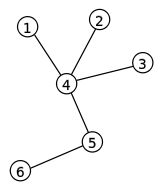
\includegraphics[height = 5cm,width = 4cm]{prufer.png}\\
上面的树结构可得普吕弗序列:{4,4,4,5}。

\subsection{从普吕弗序列还原无根树}
设这普吕弗序列长$n − 2$。首先写出数1至$n$。第一步,找出1至$n$中没有在序列中出现的最小数。把标号为这数的顶点和标号为序列首项的顶点连起来,并把这数从1至$n$中删去,序列的首项也删去。接着每一步以1至$n$中剩下的数和余下序列重复以上步骤。最后当序列用完,把1至n中最后剩下的两数的顶点连起来。

\subsection{结论}
\begin{itemize}
\item 一个长为$n−2$且每项都在1至$n$之间的序列$S$,有唯一的标号树以$S$为普吕弗序列。
\item 长$n−2$的序列共有$n^{n−2}$个,从而证明凯莱公式:$n$顶点的标号无根树共有$n^{n−2}$棵。
\item 一棵标号树实际上是标号完全图的一棵生成树。对普吕弗序列加以限制。类似的方法可以得到标号完全二分图的生成树总数。若$G$是完全二分图,一部分的顶点标号1到$n_1$,另一部分的顶点标号$n_{1} + 1$到$n$。$G$的标号生成树总数为,$n_{1}^{n_{2}-1}*n_{2}^{n_{1}-1}$其中$n_{2} = n − n_1$。
\item 普吕弗序列中某个编号$i$出现的次数$=d(i)-1,d(i)$是这个编号的节点在无根树中的度数
\item $n$个节点的度依次为$d_1, d_2,\cdots , d_n$的无根树共有 $ \frac{(n-2)!} {[ (d_1-1)!*(d_2-1)!*\cdots *(d_n-1)! ] }$个,因为此时$Prufer$编码中的数字$i$恰好出现$d_i-1$次。
\item $n$个节点的度依次为$d_1, d_2,\cdots , d_n$,另有$m$个节点度数未知,求有多少种生成树?[BZOJ1005 明明的烦恼]令每个已知度数的节点的度数为$d_i(i:1\sim k)$,有$n$个节点,$m$个节点未知度数,$sum=\sum_{i=1}^{k}(d(i)-1)$。
$$
Ans=C_{n-2}^{sum}*\frac{sum!}{\prod_{i=1}^{k}(d(i)-1)!}*(n-k)^{n-sum-2}
$$

\item $n$个点的有标号有根树的计数:$n^{n-2}*n = n^{n-1}$
\end{itemize}
\subsection{BZOJ 1211}
给定一棵$n\leq 150$个结点的树中所有点的度数,求有多少种可能的树? \\
直接乘会爆long long,所以先把每个数分解质因数,把质因数的次数相加相减,然后再乘起来。无解需要输出0。当$n!=1\&\&d[i]==0$时或者当$\sum(d[i]-1)!=n-2$时无解。
\begin{lstlisting}
int n, sum = 0;
int num[200];

ll Qpow(int a, int b) {
    ll ret = 1, t = a;
    while (b) {
        if (b & 1) ret *= t;
        t *= t;
        b >>= 1;
    }
    return ret;
}

void update(int x, int flag) {
    for (int i = 2; i * i <= x; ++i) {
        while (x % i == 0) num[i] += flag, x /= i;
    }
    if (x > 1) num[x] += flag;
}

int main() {
    scanf("%d", &n);
    for (int i = 2; i <= n - 2; ++i) update(i, 1);
    for (int i = 1; i <= n; ++i) {
        int d;
        scanf("%d", &d);
        if (d == 0 && n > 1) {
            printf("0\n");
            return 0;
        }
        sum += d;
        for (int j = 2; j <= d - 1; ++j) update(j, -1);
    }
    if (sum != 2 * n - 2) printf("0\n");
    else {
        ll ans = 1;
        for (int i = 2; i <= n; ++i) {
            if (num[i]) ans *= Qpow(i, num[i]);
        }
        printf("%lld\n", ans);
    }
    return 0;
}
\end{lstlisting}
\subsection{HDU 5629}
给$n\leq 50$个点,每个结点的度数不超过$a_i\in [1,n]$,求构造树大小(结点个数)为$s\in [1,n]$的方案数,答案对$1e9+7$取模。\\

用$dp[i][j][k]$表示处理到第$i$个节点,从中选择$j$个节点,且可重集大小(普吕弗序列长度)为$k$的排列组合数。初始化$dp[0][0][0]=1$,考虑用$dp[i-1][j][k]$来更新$dp[i][][]$的状态:不用第$i$个结点和枚举第$i$个结点的度数。滚动数组实现。\\

时间复杂度:$O(n^4)$,可以使用$FFT$优化到$O(n^3\log n)$,但是因为常数原因,差别不大。
\begin{lstlisting}
const int MAX_N = 55;
const ll mod = (ll)(1e9) + 7;

int T, n;
int a[MAX_N];
ll dp[2][MAX_N][MAX_N], C[MAX_N][MAX_N];

int main() {
    for (int i = 0; i < MAX_N; ++i) {
        C[i][0] = C[i][i] = 1;
        for (int j = 1; j < i; ++j) {
            C[i][j] = (C[i - 1][j] + C[i - 1][j - 1]) % mod;
        }
    }
    scanf("%d", &T);
    while (T--) {
        scanf("%d", &n);
        for (int i = 1; i <= n; ++i) scanf("%d", &a[i]);
        memset(dp, 0, sizeof (dp));
        dp[0][0][0] = 1;
        int now = 0;
        for (int i = 1; i <= n; ++i) {
            now ^= 1;
            memset(dp[now], 0, sizeof (dp[now]));
            for (int j = 0; j <= i; ++j) {
                for (int k = 0; k <= n - 2; ++k) {
                    dp[now][j][k] += dp[now ^ 1][j][k];
                    if (dp[now][j][k] >= mod) dp[now][j][k] -= mod;
                    for (int p = 1; p <= a[i] && k + p - 1 <= n - 2; ++p) {
            dp[now][j + 1][p + k - 1] += dp[now ^ 1][j][k] * C[k + p - 1][p - 1] % mod;
            if (dp[now][j + 1][p + k - 1] >= mod) dp[now][j + 1][p + k - 1] -= mod;
                    }
                }
            }
        }
        printf("%d", n);
        for (int j = 2; j <= n; ++j) printf(" %lld", dp[now][j][j - 2]);
        printf("\n");
    }
    return 0;
}
\end{lstlisting}

%\end{document}
